% Options for packages loaded elsewhere
\PassOptionsToPackage{unicode}{hyperref}
\PassOptionsToPackage{hyphens}{url}
%
\documentclass[
]{article}
\usepackage{amsmath,amssymb}
\usepackage{lmodern}
\usepackage{ifxetex,ifluatex}
\ifnum 0\ifxetex 1\fi\ifluatex 1\fi=0 % if pdftex
  \usepackage[T1]{fontenc}
  \usepackage[utf8]{inputenc}
  \usepackage{textcomp} % provide euro and other symbols
\else % if luatex or xetex
  \usepackage{unicode-math}
  \defaultfontfeatures{Scale=MatchLowercase}
  \defaultfontfeatures[\rmfamily]{Ligatures=TeX,Scale=1}
\fi
% Use upquote if available, for straight quotes in verbatim environments
\IfFileExists{upquote.sty}{\usepackage{upquote}}{}
\IfFileExists{microtype.sty}{% use microtype if available
  \usepackage[]{microtype}
  \UseMicrotypeSet[protrusion]{basicmath} % disable protrusion for tt fonts
}{}
\makeatletter
\@ifundefined{KOMAClassName}{% if non-KOMA class
  \IfFileExists{parskip.sty}{%
    \usepackage{parskip}
  }{% else
    \setlength{\parindent}{0pt}
    \setlength{\parskip}{6pt plus 2pt minus 1pt}}
}{% if KOMA class
  \KOMAoptions{parskip=half}}
\makeatother
\usepackage{xcolor}
\IfFileExists{xurl.sty}{\usepackage{xurl}}{} % add URL line breaks if available
\IfFileExists{bookmark.sty}{\usepackage{bookmark}}{\usepackage{hyperref}}
\hypersetup{
  pdftitle={Measuring Synchronization in Simple Neural Oscillators},
  hidelinks,
  pdfcreator={LaTeX via pandoc}}
\urlstyle{same} % disable monospaced font for URLs
\usepackage[margin=1in]{geometry}
\usepackage{longtable,booktabs,array}
\usepackage{calc} % for calculating minipage widths
% Correct order of tables after \paragraph or \subparagraph
\usepackage{etoolbox}
\makeatletter
\patchcmd\longtable{\par}{\if@noskipsec\mbox{}\fi\par}{}{}
\makeatother
% Allow footnotes in longtable head/foot
\IfFileExists{footnotehyper.sty}{\usepackage{footnotehyper}}{\usepackage{footnote}}
\makesavenoteenv{longtable}
\usepackage{graphicx}
\makeatletter
\def\maxwidth{\ifdim\Gin@nat@width>\linewidth\linewidth\else\Gin@nat@width\fi}
\def\maxheight{\ifdim\Gin@nat@height>\textheight\textheight\else\Gin@nat@height\fi}
\makeatother
% Scale images if necessary, so that they will not overflow the page
% margins by default, and it is still possible to overwrite the defaults
% using explicit options in \includegraphics[width, height, ...]{}
\setkeys{Gin}{width=\maxwidth,height=\maxheight,keepaspectratio}
% Set default figure placement to htbp
\makeatletter
\def\fps@figure{htbp}
\makeatother
\setlength{\emergencystretch}{3em} % prevent overfull lines
\providecommand{\tightlist}{%
  \setlength{\itemsep}{0pt}\setlength{\parskip}{0pt}}
\setcounter{secnumdepth}{5}
\usepackage{float} \usepackage{subcaption} \usepackage[version=4]{mhchem} \usepackage{listings} \usepackage{color}
\ifluatex
  \usepackage{selnolig}  % disable illegal ligatures
\fi
\newlength{\cslhangindent}
\setlength{\cslhangindent}{1.5em}
\newlength{\csllabelwidth}
\setlength{\csllabelwidth}{3em}
\newenvironment{CSLReferences}[2] % #1 hanging-ident, #2 entry spacing
 {% don't indent paragraphs
  \setlength{\parindent}{0pt}
  % turn on hanging indent if param 1 is 1
  \ifodd #1 \everypar{\setlength{\hangindent}{\cslhangindent}}\ignorespaces\fi
  % set entry spacing
  \ifnum #2 > 0
  \setlength{\parskip}{#2\baselineskip}
  \fi
 }%
 {}
\usepackage{calc}
\newcommand{\CSLBlock}[1]{#1\hfill\break}
\newcommand{\CSLLeftMargin}[1]{\parbox[t]{\csllabelwidth}{#1}}
\newcommand{\CSLRightInline}[1]{\parbox[t]{\linewidth - \csllabelwidth}{#1}\break}
\newcommand{\CSLIndent}[1]{\hspace{\cslhangindent}#1}

\title{Measuring Synchronization in Simple Neural Oscillators}
\author{Shivansh Dave\\
Biology Dept., Case Western Reserve University\\
\href{mailto:shivansh@case.edu}{\nolinkurl{shivansh@case.edu}}}
\date{August 10, 2020\\
~\\
\emph{To be submitted as a term paper for BIOL 419 (Spring, 2020)}}

\begin{document}
\maketitle

{
\setcounter{tocdepth}{2}
\tableofcontents
}
\newpage
\floatplacement{figure}{!htb}

\hypertarget{summary}{%
\section*{Summary}\label{summary}}
\addcontentsline{toc}{section}{Summary}

In this study, I have constructed simple neural oscillators using a pair of altered Morris-Lecar model neurons by varying different parameters such as system noise levels, synaptic connection type and neuron type (i.e., bursting/regular) to quantify and compare degree of synchrony between the two firing coupled neurons. For measuring synchronization I use two different methods (i.e., cross-correlation of raw voltage traces, and correlation using gaussian smoothed spike trains) to contrast their effectiveness for quantifying synchrony across different type of networks.

\hypertarget{introduction}{%
\section{Introduction}\label{introduction}}

Synchronization of neural firing is known to play a role in various neural phenomena. It plays an important role in memory formation. For example, tighter coupling in firing of neurons in medial temporal lobe in the brain is correlated with increased memory performance in humans and animals. In the same study it was found that neural synchronization is linked to a potential cellular mechanism for memory storage and timing-based learning tasks (Jutras and Buffalo 2010). In addition to this, synchronization is also associated with epilepsy, which affects about 3 million adults and 0.5 million children in the US and 50 million people worldwide (CDC 2018; WHO 2020). Mormann et al. (2003) found that decrease in neural synchronization precedes epileptic seizures and neural desynchronization is an immanent part of seizure initiating mechanism in humans. (Mormann et al. 2003)

Neural synchronization being an interesting topic to study, it is important to be able to understand how one can achieve synchronized firing using a simple system and to be able to quantify the synchrony in a simple neural oscillator. For an oscillator, the synchronization can be of broadly two types, namely, in-phase synchronization and anti-phase synchronization (Pikovsky and Rosenblum 2007), and different kinds of oscillator may give rise to different synchronization properties (González-Miranda 2014). For example, in certain conditions inhibitory synapse in an oscillator gives rise to synchronous firing as opposed to excitation (Van Vreeswijk, Abbott, and Bard Ermentrout 1994). In an oscillator, noise level may cause desynchronization and cause the weaker coupling between two neurons. Computational tools can allow us to construct a simple oscillator and let us study the effect of various factors such as system noise levels etc, on the degree of synchronization achieved by the oscillator.

To make neurons for oscillators, I use Morris-Lecar (ML) model, which is a reduced two-dimensional non-linear model for simulating neurons in contrast to the 4-dimensional Hodgkin--Huxley model (Lecar 2007). I use \(Ca^{2+}\) and \(K^+\) ion channels to simulate internal neuronal dynamics, as explained originally in (Morris and Lecar 1981). Now, if I connect two of such neurons to each other, would they give rise to sustained synchronous firing? and how does the degree of synchrony vary when I couple those neurons differently? This study is mainly focused on this question.

For simulating a simple oscillator, I use a half-center oscillator (HCO) made through synaptically connecting two ML neurons reciprocally with each other. Since different types of oscillators give rise to different oscillation patterns, I use many different HCOs (See section \ref{hco}), made by varying the type of synapses and neurons. To get a bursting type HCO, I altered the ML neurons to remove their dependence on external stimulation current for initiating spikes. These bursting ML neurons have slow internal feedback current, responsible for their bursting properties (Mainen and Sejnowski 1996).

How synchronized is an oscillator for a given noise level in the neurons? To be able to study effects of noise (which can represent physical phenomenon such as ambient temperature, etc.), I stochastically simulate operation of both the ion channels and compare the synchronization of stochastically simulated HCO to the deterministic simulations. The smaller the count of ion channels present in a neuron, the larger the noise levels will be for that system. Thus, I vary system size (i.e., \(\Omega\)) for each ion channel for quantifying their effects on synchronization.

\hypertarget{methods}{%
\section{Methods}\label{methods}}

I used the Morris--Lecar (ML) model as a base for making my neurons for deterministic simulations (See Section \ref{MLdt}). I altered the model parameters to get the ion channels (i.e., K+ and Ca2+) to operate stochastically (see \ref{MLst}) by modeling the Chemical Langevin Equations for a first order single variable chemical reaction (see \ref{CLE}). The altered ion channel properties and a slow internal feedback current are used for making the ML neurons to operate in the ``bursting mode'' (see \ref{Bpar}).

Chemical synapses of the type excitatory as well as inhibitory are achieved by introducing the synapses on ML neurons (see \ref{syn}). Two ML neurons of any type (i.e., deterministic/stochastic and plain/bursting) are reciprocally connected to each other using chemical synapses (i.e., excitatory or inhibitory) to get the functioning Half center oscillator (HCO), (see \ref{hco}). The HCO shows a varied degree of synchronizations based on the type of neurons and the connections. I employ and compare both, the gaussian smoothed spike-time method (see \ref{blc}) and the Pearson's linear correlation of raw voltage traces, to compare the degree of synchronization between the participating ML neurons in various types of HCOs.

\hypertarget{ML}{%
\subsection{ML Neurons}\label{ML}}

I am simulating an array of altered Morris-Lecar neurons (i.e., ML neurons) in parallel to find the next membrane voltage and the ion channel states using the present conditions using a Matlab script I wrote for this purpose (see \ref{MLm}). Any of these neurons can receive a chemical synapse and project a chemical synapse onto any other neuron connected in the network. The Matlab simulation script (with a ``demo'' network) is used for initializing and simulating the network for a given duration (see Appendix \ref{MLm}).

This section contains the details on the mathematical and computational tools used for basic operational realization of ML neurons. Subsequent sections will cover any further modifications such as introducing synapses (see \ref{syn}) and enabling slow internal feedback current for bursting mode (see \ref{Bpar}).

\hypertarget{MLdt}{%
\subsubsection{Deterministic Neuron}\label{MLdt}}

Firstly, to achieve deterministic simulation of ML neurons I used equations \eqref{eq:dvdt}-\eqref{eq:tau}, and used some constant parameters \eqref{eq:par}, which I referred from (Anderson, Ermentrout, and Thomas 2015; Lecar 2007).

\begin{figure}
  \captionsetup[subfigure]{labelformat=empty} \centering
  \begin{subfigure}[b]{0.75\textwidth}
    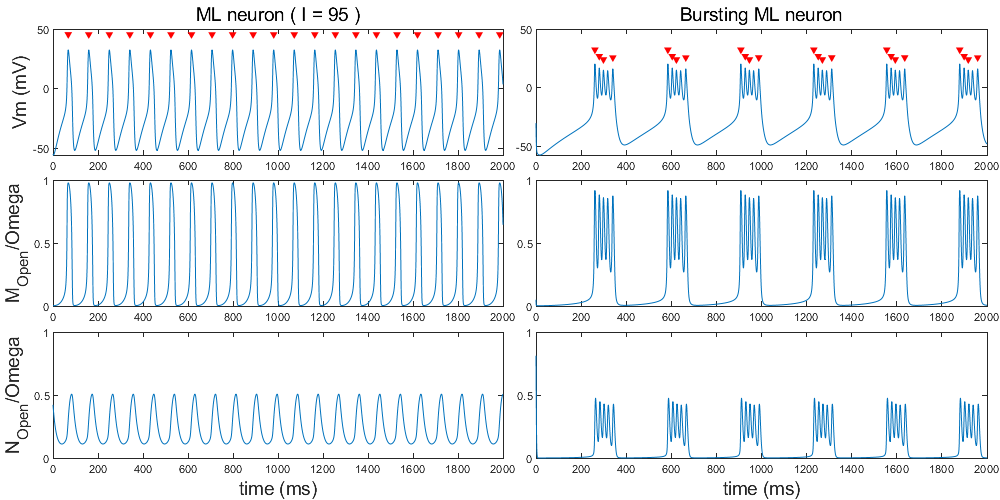
\includegraphics[width=\textwidth]{figs/F0_A_ML_channel_det.png}
    \caption{} \label{fig:fig0dt}
  \end{subfigure}
  \vspace{-0.75cm}
  \caption{(A) Deterministic ML Neuron membrane voltage and activation of $K^+$ and $Ca^{2+}$ ion channels, (left) in plain/regular ML neurons; (right) ML neurons with bursting mode.}
\end{figure}

\begin{align} 
\label{eq:dvdt} \frac{dv}{dt} = f(v,n) = 
    \frac1C ( I_{\rm app} - &g_{\rm Ca} m_\infty (v) (v - v_{\rm Ca}) - 
    g_{\rm K} n (v - v_{\rm K}) - g_{\rm L}(v - v_{\rm L}) ) \\
\nonumber \frac{dn}{dt}  =  g(v,n) &= \alpha(v)(1-n) - \beta(v)n \\
\label{eq:dndt} &= (n_\infty(v)-n)/\tau(v)
\end{align}

Equation \eqref{eq:dvdt} shows the deterministic membrane voltage for the ML model neurons. In which, \(n; (n \in [0,1])\) represents a fraction of \(K^+\) ion channels open at the given time \(t\). \(I_{\rm app}\) is the current value, measured in \(\mu A/cm^2\), which can represent either the current-clamp current (i.e, \(I_{stim}\)) in case of regular or plain ML neurons (left in Figure\ref{fig:fig0dt}) or it can represent the slow internal feedback current (i.e., \(I_{internal}\)) for the bursting mode ML neurons (see \ref{Bpar}; right plots in Figure\ref{fig:fig0dt}). Eq.\eqref{eq:dndt} represents the dynamical opening of \(K^+\) ion channels which depends on \(\alpha\) and \(\beta\), which are the \emph{per capita} transition rates of ion channels to open or close dynamically \eqref{eq:ab}. ALternatively, the dynamic operation of \(n\) can be computed by the steady-state value of \(n\) (i.e., the fraction of \(K^+\) ion channels open in steady-state) and temporal dynamics of the recovery process of channel operation, \(\tau\), as shown in \eqref{eq:dndt}. The values of \(\alpha, \beta, n_\infty\) and \(\tau\) depend on a present value of membrane voltage, \(v\), and can be modeled using the voltage constants (i.e., \(v_c, v_d\)). For convenience, a membrane voltage dependent variable, \(\xi\), is defined \eqref{eq:ab}. The voltage constants \(v_a\) and \(v_b\) are used to model membrane voltage dependent dynamic operation of \(Ca^{2+}\) ion channels.

\begin{align}
\nonumber \phi=0.04\ s^{-1},\ v_a&=-1.2\ mV,\ v_b=18\ mV,\ v_c=2\ mV,\ v_d=30\ mV,
\\ \label{eq:ab} \xi = \frac{v-v_c}{v_d},\ 
    &\alpha(v) = \frac{\phi \cosh(\xi/2)}{1+ e^{2\xi}},\ 
    \beta(v) = \frac{\phi \cosh(\xi/2)}{1+ e^{-2\xi}},
\\ \label{eq:nss} n_\infty(v) &= \frac{\alpha(v)}{\alpha(v) + \beta(v)} \ 
    =\  \frac12(1 + \tanh \xi)
\\ \label{eq:mss} m_\infty &= \frac12\left(1+ \tanh(\frac{v-v_a}{vb})\right)
\\ \label{eq:tau} \tau(v) &= \frac{1}{\alpha(v) + \beta(v)} \ 
    =\  \frac{1}{\phi \cosh(\xi/2)}
\end{align}

Other fixed constants used for deterministic simulations are listed below \eqref{eq:par}. Ion channel maximum conductance \(g_{\rm K}, g_{\rm Ca}\ and\ g_{\rm L}\) are for \(K^+, Ca^{2+}\) and leak channels respectively, which are measured in \(m\mho/cm^2\). Reversal potentials for these ion channels (i.e., \(v_{\rm K},\ v_{\rm Ca},\ v_{\rm L}\)) and other voltage constants (i.e., \(v_{a,b,c,d}\)) are measured in mV. \(\phi\), measured in \(s^{-1}\) is a rate constant for the recovery process of \(K^+\) ion channels. \(v_a\) and \(v_c\) are the voltages at which the ion channel activation function \(m_{\infty}\) and \(n_{\infty}\), respectively, becomes 0.5; and \(v_b\) and \(v_d\), respectively, are the slope values for those membrane voltage dependent functions. \(C\) is the membrane capacitance measured in \(\mu F/cm^2\). (Morris and Lecar 1981)

\begin{equation} \label{eq:par}
\begin{split}
&v_{\rm Ca} = 120\ mV,\  v_{\rm K} = -84\ mV,\ v_{\rm L} = -60\ mV,
\\ &g_{\rm Ca} = 4.4\ m\mho/cm^2, \ g_{K\rm } = 8\ m\mho/cm^2,\ 
    g_{\rm L} = 2\ m\mho/cm^2,
\\ &C = 20\ \mu F/cm^2,\ I_{\rm app} = (variable;\ measured\ in\ 
    \mu A/cm^2) 
\end{split}
\end{equation}

Using the equations \eqref{eq:dvdt}-\eqref{eq:par}, by applying \(I_{\rm app}=I_{stim} = 95\), I see the membrane voltage and ion channels as shown in the left in Figure \ref{fig:fig0dt}. Red-markers indicate the identified spikes in the membrane voltage traces (see \ref{spk}). The signal in the second is normalized \(Ca^{2+}\) ion channel activation computed using \(m_{\infty}\) and the signal in the third row represents the normalized activation of \(K^+\) ion channels (i.e., \(n, n\in[0,1]\)), computed using equation \eqref{eq:dndt}. Bursting mode ML neurons show fast and slow dynamics, that is the fast spikes for action potential and the slow oscillation of \emph{plateau potential}, more details on the simulation parameters are given in section \ref{Bpar}.

\hypertarget{MLst}{%
\subsubsection{Stochastic ML Neuron}\label{MLst}}

Stochastic activation of both, the \(K^+\) and \(Ca^{2+}\), ion-channels are used for simulation of ML neurons and to compute membrane voltage (Figure \ref{fig:fig0st}). For the simulation I used the following equations \eqref{eq:stdv}-\eqref{eq:nt}, and used constant parameters \eqref{eq:stpar} for the ML neurons, as described in (Anderson, Ermentrout, and Thomas 2015).

\begin{figure}    \ContinuedFloat
  \captionsetup[subfigure]{labelformat=empty} \centering
  \begin{subfigure}[b]{0.75\textwidth}
    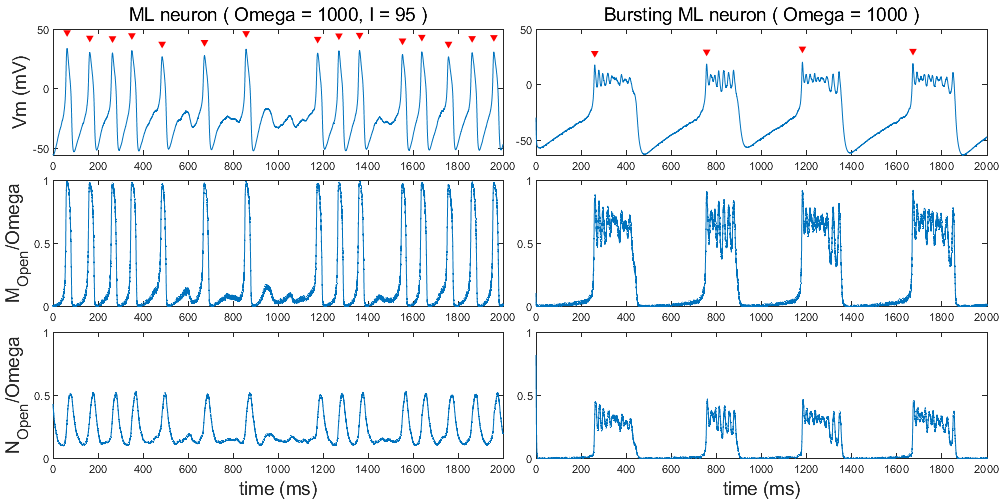
\includegraphics[width=\textwidth]{figs/F0_B_ML_channel_stoch.png}
    \caption{} \label{fig:fig0st}
  \end{subfigure}
  \vspace{-0.75cm}
  \caption{(B) Stochastic ML Neuron membrane voltage and Stochastic activation of $K^+$ and $Ca^{2+}$ ion channels, (left) in plain/regular ML neurons; (right) ML neurons with bursting mode.}
\end{figure}

Equation \eqref{eq:stdv} shows the stochastic membrane voltage for the ML model neurons with \(n\) and \(m\); \((n,m \in [0,1])\) represents the fraction of \(K^+\) and \(Ca^{2+}\) ion channels open at the given time \(t\). Both of which depend on the instantaneous membrane voltage of the ML neuron Eq. \eqref{eq:stdn}-\eqref{eq:stdm}. Stochastic activation of \(K^+\) and \(Ca^{2+}\) ion channels depends on the \emph{per capita} transition rates \(\alpha_n,\beta_n\) and \(\alpha_m,\beta_m\), respectively {[}\eqref{eq:ma}, \eqref{eq:mb}, \eqref{eq:na}, \eqref{eq:nb}{]}. Same as the deterministic equations, the \(I_{\rm app}\) (\(\mu A/cm^2\)) represents either the current-clamp current (i.e, \(I_{stim}\)) in case of regular or plain ML neurons (left, in Figure \ref{fig:fig0st}) or the slow internal feedback current (i.e., \(I_{internal}\)) for the bursting mode ML neurons (see \ref{Bpar}; right plots, in Figure \ref{fig:fig0st}).

\begin{align} 
\label{eq:stdv} \frac{dv}{dt} = F(v,n,m) &= \frac1C ( I_{\rm app} - 
    g_{\rm Ca} m (v - v_{\rm Ca}) - g_{\rm K} n (v - v_{\rm K}) - 
    g_{\rm L}(v - v_{\rm L}) )
\\ \nonumber \frac{dn}{dt}  =  G(v,n, m) &= \alpha_n(v)(1-n) - \beta_n(v)n 
\\ \label{eq:stdn} &= (n_\infty(v)-n)/\tau_n(v)
\\ \nonumber \frac{dm}{dt}  =  H(v,n, m) &= \alpha_m(v)(1-m) - \beta_m(v)m 
\\ \label{eq:stdm} &= (m_\infty(v)-m)/\tau_m(v)
\end{align}

Cell voltage dependent functions of \(\alpha_m, \beta_m, \tau_m\) and \(m_\infty\) are modeled using the voltage constants (i.e., \(v_a, v_b\) (mV)) and recovery process rate constant \(\phi_m\ (s^{-1})\) for stochastic operation of \(Ca^{2+}\) ion channels. The activation threshold (i.e., \(n=0.5\)) and the slope of the voltage dependent activation function, \(n_{\infty}\) is set by \(V_a\) and \(v_b\), respectively. For convenience, a membrane voltage dependent variable, \(\xi_m\), is defined using \(v_a, v_b\) {[}Equations \eqref{eq:mxi}-\eqref{eq:mt}{]}.

\begin{align}
\nonumber \phi_m = 2\ s^{-1},\  v_a &= -1.2\ mV,\ v_b = 18\ mV,
\\ \label{eq:mxi} \xi_m &= \frac{v-v_a}{v_b},
\\ \label{eq:ma} \alpha_m(v) &= \frac{\phi_m \cosh(\xi_m/2)}{1+ e^{2\xi_m}},
\\ \label{eq:mb} \beta_m(v) &= \frac{\phi_m \cosh(\xi_m/2)}{1+ e^{-2\xi_m}},
\\ \nonumber  m_\infty(v) &= \frac{\alpha_m(v)}{\alpha_m(v) + \beta_m(v)} 
\\ \label{eq:minf} &= \frac12(1 + \tanh \xi_m) 
\\ \nonumber \tau_m(v) &= \frac{1}{\alpha_m(v) + \beta_m(v)} 
\\ \label{eq:mt} &= \frac{1}{\phi \cosh(\xi_m/2)}
\end{align}

Same as the \(Ca^{2+}\) channels, the \(K^{+}\) channels are stochastically simulated using voltage dependent functions such as \(\alpha_n, \beta_n, \tau_n\) and \(n_\infty\). These functions are modeled using the voltage constants (i.e., \(v_c, v_d\) (mV)) and rate constant \(\phi_n\ (s^{-1})\) and for convenience, a membrane voltage dependent variable, \(\xi_n\), is defined using \(v_c, v_d\) {[}Equations \eqref{eq:nxi}-\eqref{eq:nt}{]}. \(v_c\) sets the activation threshold (i.e., \(n=0.5\)) and \(v_d\) sets the slope of the voltage dependent activation function, \(n_{\infty}\).

\begin{align} 
\nonumber \phi_n = 0.04\ s^{-1},\ v_c &= 2\ mV,\ v_d = 30\ mV,
\\ \label{eq:nxi} \xi_n &= \frac{v-v_c}{v_d},
\\ \label{eq:na} \alpha_n(v) &= \frac{\phi_n \cosh(\xi_n/2)}{1+ e^{2\xi_n}},
\\ \label{eq:nb} \beta_n(v) &= \frac{\phi_n \cosh(\xi_n/2)}{1+ e^{-2\xi_n}},
\\ \nonumber n_\infty(v) &= \frac{\alpha_n(v)}{\alpha_n(v) + \beta_n(v)} 
\\ \label{eq:inf} &= \frac12(1 + \tanh \xi_n) 
\\ \nonumber \tau_n(v) &= \frac{1}{\alpha_n(v) + \beta_n(v)} 
\\ \label{eq:nt} &= \frac{1}{\phi \cosh(\xi_n/2)}
\end{align}

The stochastic ML neuron constants \eqref{eq:stpar} such as reversal potentials, conductance and capacitance are set exactly the same as deterministic parameters \eqref{eq:par}. (Morris and Lecar 1981; Anderson, Ermentrout, and Thomas 2015)

\begin{equation} \label{eq:stpar}
\begin{split}
&v_{\rm Ca} = 120\ mV,\  v_{\rm K} = -84\ mV,\ v_{\rm L} = -60\ mV,
\\ &g_{\rm Ca} = 4.4\ m\mho/cm^2, \ g_{K\rm } = 8\ m\mho/cm^2,\ 
    g_{\rm L} = 2\ m\mho/cm^2,
\\ &C = 20\ \mu F/cm^2,\ I_{\rm app} = (variable;\ measured\ in\ 
    \mu A/cm^2) 
\end{split}
\end{equation}

Figure \ref{fig:fig0st} is an example simulation of stochastically activating \(Ca^{2+}\) and \(K^+\) ion channels (displayed in the second and third rows, respectively) using the equations \eqref{eq:stdv}-\eqref{eq:stpar}. For that purpose system size (i.e., \(\Omega_{N,M}\)) for both ion channels is set to 1000 and for the plain neurons (on the left) are made to spontaneously spike action potentials by applying \(I_{\rm app}=I_{stim} = 95\) with red-markers to indicate the identified spikes in the membrane voltage traces (see \ref{spk}). Stochastic ML neurons in bursting mode are explained in section \ref{Bpar}. The following section, \ref{CLE} shows the derived model using Langevin equations for simulating these neurons.

\hypertarget{CLE}{%
\subsubsection{Setting up Chemical Langevin Equation}\label{CLE}}

In the study both the ion channels in ML neurons, \(K^+\) and \(Ca^{2+}\) channels are operating stochastically for the stochastic simulations. I use Chemical Langevin Equations (CLE) to simulate ion channels stochastically. This method is an approximation method and uses Stochastic Differential Equations (SDE) for stochastic simulation, which is faster than other approximation methods like \(\tau\)-leaping and the exact methods like Gillespie's exact method (Higham 2008). To speed up computation CLE uses diffusion approximation in addition to time approximations used in \(\tau\)-leaping method, and with faster reaction rates, to get sufficiently large number of reactions happening (for each species), the errors incur would be small by switching to CLE as compared to other exact methods (Wilkinson 2019).

As shown in \eqref{eq:rxn}, for each ion channels (for each different ions involved in the simulation, i.e., \(K^+, Ca^{2+}\) for ML neurons) I can compare it to a first order reaction chemical reaction showing the rates of switching the states between ``open'' and ``close.'' (Note : Here \(N_{open}, N_{close}\) shows the states for \(K^+\) ion channels, and similarly one can get another sets of equations for \(Ca^{2+}\) ion channels represented by \(M_{open},M_{close}\).). Similar method is present for Hodgkin--Huxley model in (Ermentrout and Terman 2010).

\begin{equation} \label{eq:rxn} 
\ce{ N_{close} <=>[\alpha][\beta] N_{open} }
\end{equation}

From \eqref{eq:rxn}, two sub-reactions can be formulated along with a stoichiometry matrix for each sub-reaction. \eqref{eq:rxn1} and \eqref{eq:rxn2} shows the chemical hazard function for channel opening and closing reactions.

\begin{equation} \label{eq:rxn1}
\begin{split}
Reaction\ (1): \ce{ N_{close} ->[\alpha] N_{open} },
\\ h_1(N) = \alpha N_{close}\ ;\ \ \ \zeta_1=\binom{-1}{+1}  
\end{split}
\end{equation}

\begin{equation} \label{eq:rxn2}
\begin{split}
Reaction\ (2): \ce{ N_{open} ->[\beta] N_{close} },
\\ h_2(N) = \beta N_{open}\ ;\ \ \zeta_2=\binom{+1}{-1}
\end{split}
\end{equation}

Since in my model, mass conservation is applicable as no immigration/birth/death are not happening, for simplifying the computation, I can convert 2D sets of equations to 1D equations. Total count for \(K^+\) ion channels in the simulation is denoted by \(\Omega_N\) (similarly \(\Omega_M\) for \(Ca^{2+}\) channels). \(N(t)\) represents the count of channels in \(N_{open}\) state at a given time, \(t\), so the count of channels in \(N_{close}\) state would be \(\Omega_N - N(t)\) at that time. I then updated the reaction hazard function for 1D system \eqref{eq:1d}.

\begin{equation} \label{eq:1d}
\begin{split}
\Omega_N = N_{open} + &N_{close}\ ;\ \ N(t) = N_{open}(t)
\\ \therefore\ N_{close}(t) &= \Omega_N - N_{open}(t) 
\\ h_{1(N)} & = \alpha (\Omega_N - N)
\\ h_{2(N)} &= \beta N 
\end{split}
\end{equation}

Chemical Langevin Equations can be set up as described (Higham 2008; Wilkinson 2019) for ion channel simulation. For each time step of \(\tau\), the state of each ion channels counts can be updated using the following equation :

\begin{equation}
\begin{split}
N(t+\tau) = N(t) &+ \tau (h_{1(N)}-h_{2(N)}) 
\\ &+ \sqrt{\tau\  h_{1(N)}}\ \xi_1(t) 
\\ &- \sqrt{\tau\  h_{2(N)}}\ \xi_2(t)\ ;\ \ \xi_{1,2}(t) \sim \mathcal{N}(0,1)
\\ \implies N(t+\tau) = N(t) &+ \tau (h_{1(N)}-h_{2(N)}) 
\\ &+ \sqrt{\tau} \sqrt{h_{1(N)}+h_{2(N)}}\ \xi(t)\ ;\ \ \xi(t) \sim \mathcal{N}(0,1)
\end{split}
\end{equation}

I use \eqref{eq:dv}-\eqref{eq:M} for simulating simple ML neurons (Figure \ref{fig:fig0st}) to update each ion channel stochastically using CLE.

\begin{align}
\label{eq:dv} \frac{dV}{dt} =  F(V(t),N(t),M(t)) &= \frac1C ( I_{\rm app} - g_{\rm Ca} 
    \frac{M(t)}{\Omega_M} \left(V(t) - v_{\rm Ca}\right) - g_{\rm K} 
    \frac{N(t)}{\Omega_N} \left(V(t) - v_{\rm K}\right) - g_{\rm L}(V - v_{\rm L}) )
\\ \nonumber N(t+\tau) = N(t) &+ \tau (\alpha (\Omega_N - N(t)) - \beta N(t)) 
\\ \label{eq:N} &+ \sqrt{\tau} \sqrt{\alpha (\Omega_N - N(t)) + \beta N(t)}\ \xi_N(t)
\\ \nonumber M(t+\tau) = M(t) &+ \tau (\alpha (\Omega_M - M(t)) - \beta M(t)) 
\\ \label{eq:M} &+ \sqrt{\tau} \sqrt{\alpha (\Omega_M - M(t)) + \beta M(t)}\ \xi_M(t)\ ;
    \ \ \ \xi_{N,M}(t) \sim \mathcal{N}(0,1)
\end{align}

Values of other parameters and constants are as described earlier in \ref{MLst}. Also, see \ref{syn} for the equations with adding chemical synapse used for simulation of HCOs.

\hypertarget{Bpar}{%
\subsubsection{Bursting mode in ML Neurons}\label{Bpar}}

ML Neurons explained in previous sections were plain/regular neurons (i.e., non-bursting), where input current is the current clamp current (i.e., \(I_{\rm app} = I_{stim}\)). But, I also used ML neurons in bursting mode (right side in Figure \ref{fig:fig0dt} \& \ref{fig:fig0st}). In bursting mode, the Current clamp current is set to zero (i.e., \(I_{stim}=0\)) and a slow feedback current internal current, computed as \eqref{eq:Bi}, is responsible for \emph{plateau potential} and reaching the action potential firing threshold is responsible for fast dynamics of spikes (Izhikevich 2006). For bursting mode, I used the following parameters, which I found suitable to elicit fast and slow dynamics present in this mode.

\begin{align} 
\nonumber I_{\rm app} &= I_{internal}
\\ \nonumber \varepsilon = 0.01&;\ v_o = -26;
\\ \label{eq:Bi} \frac{dI_{internal}}{dt} = &\varepsilon*(v_o - V(t))
\end{align}

For simulating ion channels most of the ML neuron parameters and constants are used as described in the previous section (For deterministic simulation \eqref{eq:par}; stochastic simulation \eqref{eq:stpar}). The changes in the parameters are shown as below.

For achieving bursting mode in deterministic simulation (right side, Figure \ref{fig:fig0dt}), the changes made are shown in \eqref{eq:Bpar}.

\begin{equation} \label{eq:Bpar}
\begin{split}
\phi=0.23,\ v_c = 12,\ v_d = 17.4
\end{split}
\end{equation}

Similarly, for bursting mode in stochastic simulation (right side, Figure \ref{fig:fig0st}), the changes in parameters are shown in \eqref{eq:Bparst}.

\begin{equation} \label{eq:Bparst}
\begin{split}
\phi_m=2,\ \phi_n=0.23,\ v_c = 12,\ v_d = 17.4
\end{split}
\end{equation}

Detailed description on designing different types of neurons is given in (Rinzel and Ermentrout 1998).

\hypertarget{effect-of-current-and-noise}{%
\subsection{Effect of Current and Noise}\label{effect-of-current-and-noise}}

Stimulus current would change the output of regular ML neurons and change in system size would affect the noise level in both the types of ML neurons, regular and bursting mode.

\hypertarget{varying-current-and-system-sizein-plain-ml-neurons}{%
\subsubsection{Varying current and system sizeIn plain ML neurons}\label{varying-current-and-system-sizein-plain-ml-neurons}}

\begin{figure}
  \captionsetup[subfigure]{labelformat=empty} \centering
  \begin{subfigure}[b]{\textwidth}
    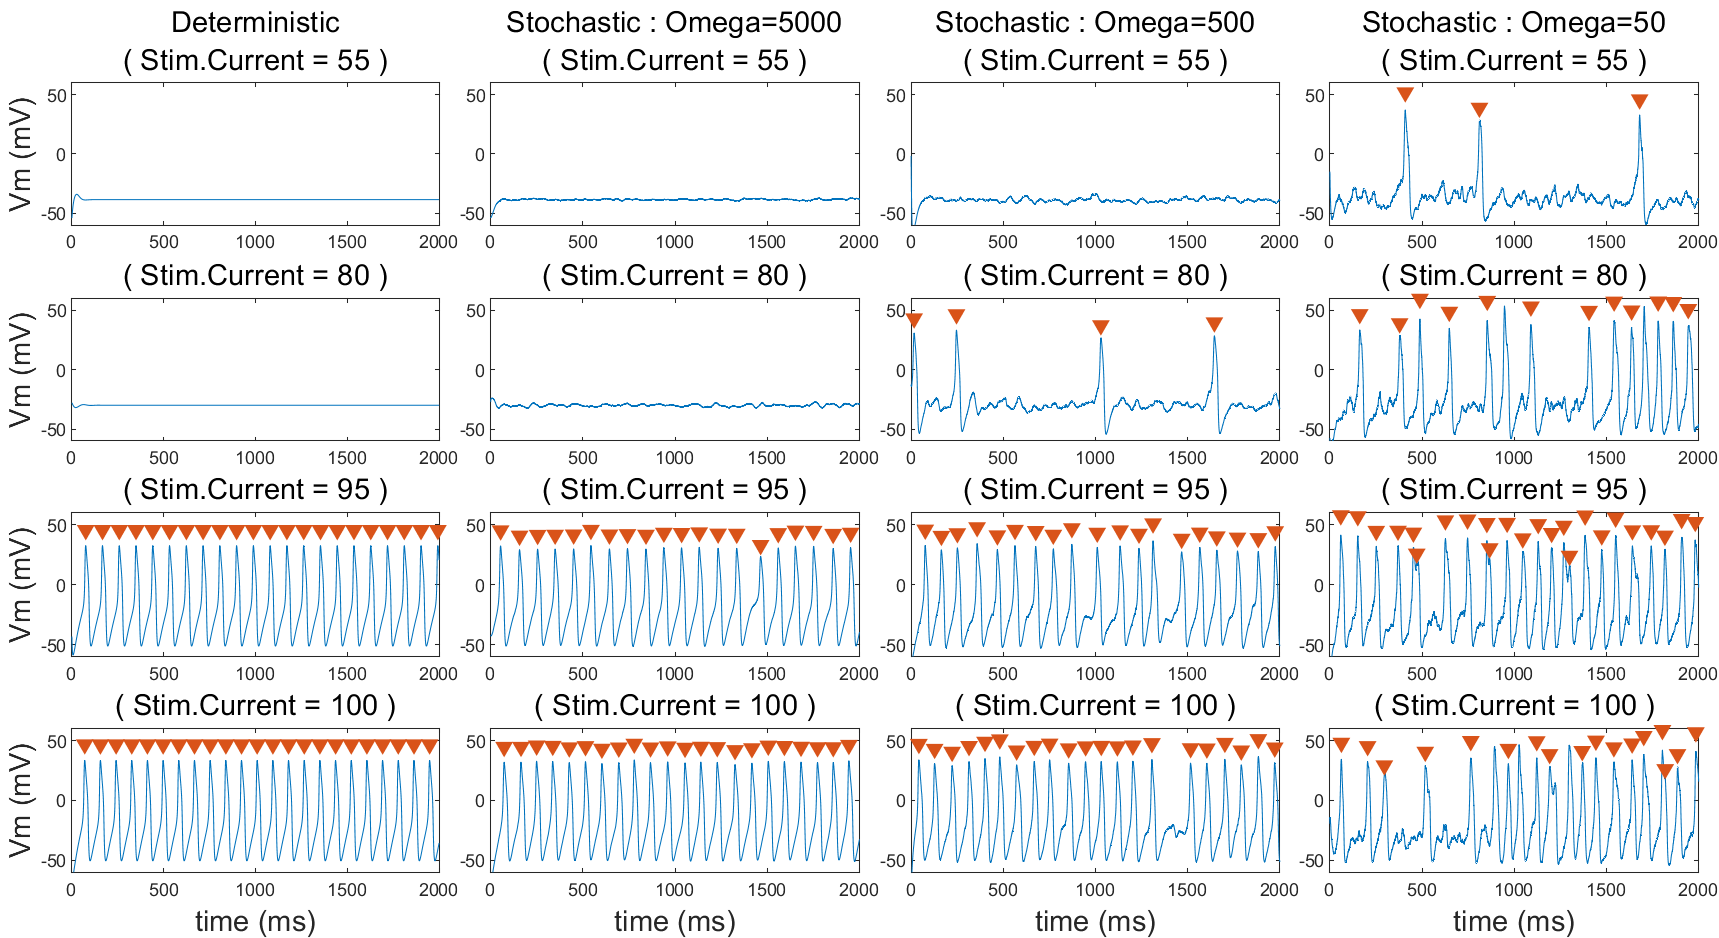
\includegraphics[width=\textwidth]{figs/F1_A_ML_Omega_Current.png}
    \caption{} \label{fig:fig1nb}
  \end{subfigure}
  \vspace{-1cm}
  \caption{(A) Plain (non-bursting) ML neurons for different system size and stim. current.}
\end{figure}

Figure \ref{fig:fig1nb} shows regular ML neurons changing behavior with varied current (along the column) and the noise (along the row). Threshold amount of stimulus current for deterministic neurons to start firing is about 89 \(\mu A/cm^2\). For stochastic neurons, increasing noise (i.e., reducing \(\Omega\)) allows more spontaneous spikes for sub-threshold stimulus currents.

\hypertarget{in-bursting-mode}{%
\subsubsection{In Bursting mode}\label{in-bursting-mode}}

\begin{figure}    \ContinuedFloat
  \captionsetup[subfigure]{labelformat=empty} \centering
  \begin{subfigure}[b]{0.6\textwidth}
    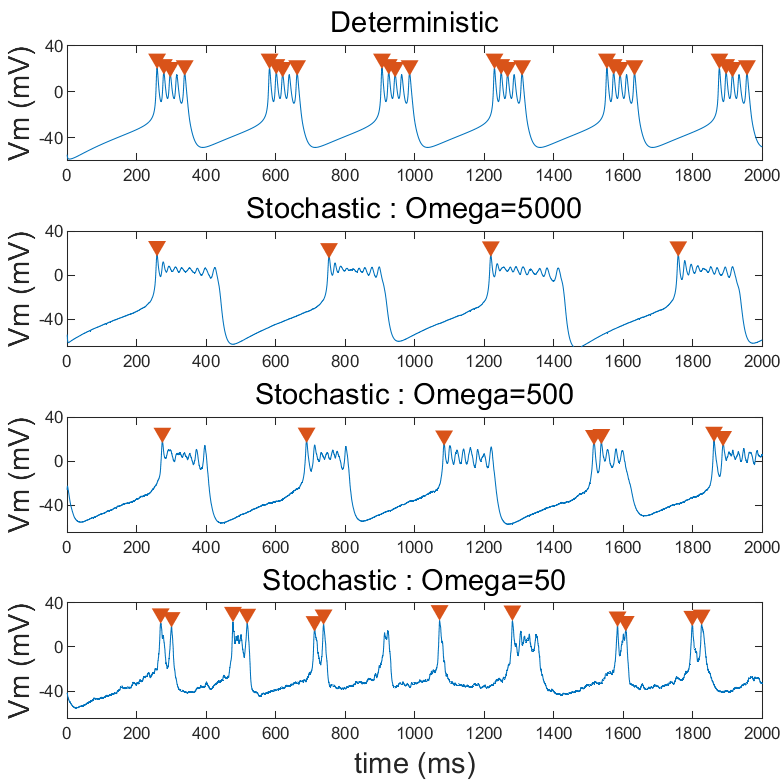
\includegraphics[width=\textwidth]{figs/F1_B_ML_Omega_Bursting.png}
    \caption{} \label{fig:fig1b}
  \end{subfigure}
  \vspace{-0.75cm}
  \caption{(B) ML neurons in bursting mode with different system size. No external stimulus current is provided here.}
\end{figure}

Figure \ref{fig:fig1b} shows Bursting mode ML neurons under various noise levels. Changing noise levels affects the rhythm and bursting dynamics of ML neurons. Increasing noise increases bursting frequency in such neurons.

To summarize, higher system size in stochastic simulation causes lower noise, and the resulting patterns look more comparable to deterministic simulations. Also, for regular neurons, increasing current causes frequent firing of spikes. Effects of noise are drastic in lower current simulations.

\hypertarget{syn}{%
\subsection{Adding Synapse}\label{syn}}

To be able to create a network out of ML neurons, I altered the ML model neurons, once again, to have a chemical synapse of both the inhibitory and excitatory types. Each neuron in the array of network, can be configured separately to receive either no-synapse, inhibitory or excitatory synapses from a desired neuron from the network (Appendix \ref{MLnet}).

\hypertarget{activation-function}{%
\subsubsection{Activation function}\label{activation-function}}

\begin{figure}
  \captionsetup[subfigure]{labelformat=empty} \centering
  \begin{subfigure}[b]{0.5\textwidth}
      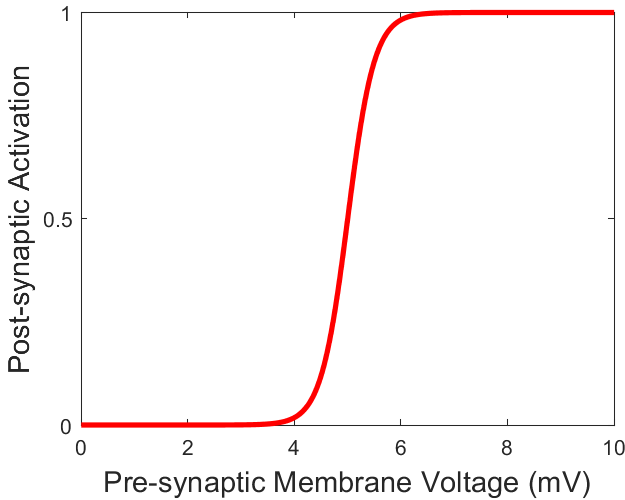
\includegraphics[width=\textwidth]{figs/F2_A_ML_Synapse_ActFxn.png}
      \caption{} \label{fig:fig2act}
  \end{subfigure}
  \vspace{-0.75cm}
  \caption{(A) Synaptic Activation Function}
\end{figure}

Figure \ref{fig:fig2act} shows the activation function with a synaptic threshold of +5 mV and the function slope of 0.5. I used \eqref{eq:actsyn} to define the sigmoidal activation function, which is inspired from (Yu and Thomas, n.d.).

\begin{equation} \label{eq:actsyn}
\begin{split}
syn_{Threshold} = 5,\ &syn_{Slope} = 0.5, 
\\ S_{syn}(v) = \frac12(1+\tanh ((v-&syn_{Threshold})/syn_{Slope}));
\end{split}
\end{equation}

\hypertarget{synaptic-current}{%
\subsubsection{Synaptic current}\label{synaptic-current}}

Synaptic current (measured in \(\mu A/cm^2\)) is computed using the following formula for Inhibitory and excitatory synapses in \eqref{eq:isyn}.

\begin{equation} \label{eq:isyn}
\begin{split}
v_{\rm syn}(exci.) = 100\ mV,\ &v_{\rm syn}(inhi.) = -100\ mV,\ g_{\rm syn} = 1\ m\mho/cm^2
\\ I_{\rm syn}(v) = &-g_{\rm syn}S_{syn}(v)(v-v_{\rm syn})\ \ \mu A/cm^2
\end{split}
\end{equation}

Synaptic current is added in in \(I_{\rm app}\) along with other possible currents such as current clamp current, \(I_{stim}\), or the internal feedback current \(I_{internal}\). Thus, for regular ML neurons with synapse will become as following,

\begin{equation} \label{eq:addsyn}
\begin{split}
(For\ plain\ ML\ neuron\ with\ Synapse)\ \ I_{\rm app} &= I_{stim} + I_{\rm syn}(v)
\\ (For\ bursting\ ML\ neuron\ with\ Synapse)\ \ I_{\rm app} &= I_{internal} + I_{\rm syn}(v)
\end{split}
\end{equation}

\hypertarget{synapses-in-deterministic-simulation}{%
\paragraph{Synapses in deterministic simulation}\label{synapses-in-deterministic-simulation}}

\begin{figure}  \ContinuedFloat
  \captionsetup[subfigure]{labelformat=empty} \centering
  \begin{subfigure}[b]{\textwidth}
      \caption{} \label{fig:fig2dt}
      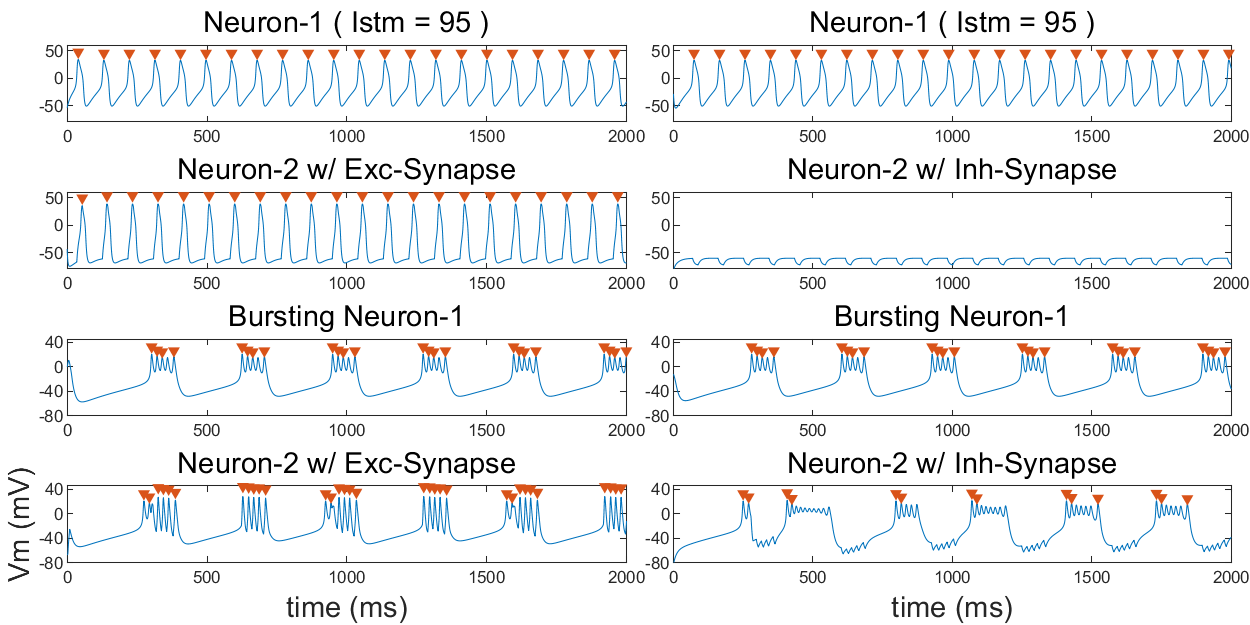
\includegraphics[width=\textwidth]{figs/F2_B_ML_Synapse_Deter.png}
  \end{subfigure}
  \vspace{-0.5cm}
  \caption{(B) Synaptic operations in deterministic ML neurons}
\end{figure}

Figure \ref{fig:fig2dt} shows the effect of a synapse in deterministic ML neurons in regular and bursting mode with the synapse is formed on Neuron-2. Regular type Neuron-1 are having current clamp, \(I_{stim}=95\) to elicit spontaneous spikes in Neuron-1. Neuron-2 is left unconnected for both the cases to see the effect of presynaptic activity.

\hypertarget{synapses-in-stochastic-simulation}{%
\paragraph{Synapses in stochastic simulation}\label{synapses-in-stochastic-simulation}}

\begin{figure}    \ContinuedFloat
  \captionsetup[subfigure]{labelformat=empty} \centering
  \begin{subfigure}[b]{\textwidth}
      \caption{} \label{fig:fig2st}
      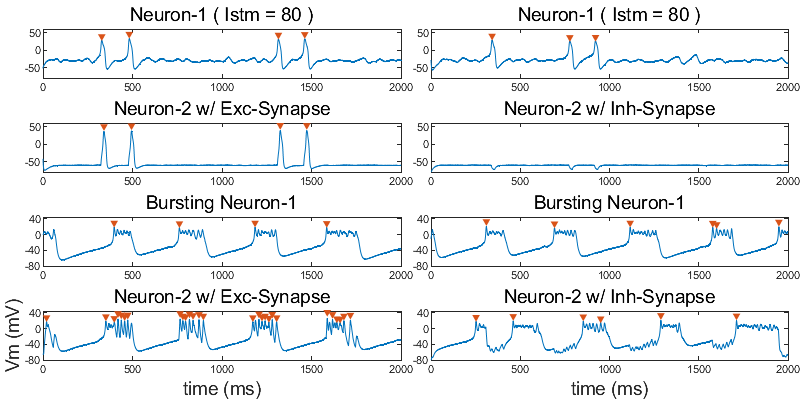
\includegraphics[width=\textwidth]{figs/F2_C_ML_Synapse_Stoch.png}
  \end{subfigure}
  \vspace{-0.5cm}
  \caption{(C) Synaptic operations in deterministic and stochastic ML neurons}
\end{figure}

Figure \ref{fig:fig2st} shows synapse in stochastic ML neurons with \(\Omega_{M,N}=500\) for all neurons. Neuron-1 (regular type) are firing action potentials due to the current clamp stimulus current \(I_{stim}=80\) and the bursting neurons (at the bottom of the image), show the firing due to internal feedback current. Each of the ``driving'' neuron is labeled as Neuron-1, which is projecting a synapse onto Neuron-2 via either excitatory (left-column) or inhibitory (right-column) chemical synapse. Figure \ref{fig:fig2st} displays stochastic neurons.

\hypertarget{hco}{%
\subsection{Half Center Oscillator}\label{hco}}

Half center oscillator is formed through a reciprocal connection of two ML neurons and each of them are supplied with super-threshold stimulus current in case of plain ML neuron types. So combining the type of synapse type of ML neuron, I get the following types of HCOs :

\begin{enumerate}
\def\labelenumi{\arabic{enumi}.}
\tightlist
\item
  Excitatory HCO with ML neurons, i.e, e-HCO(1)
\item
  Inhibitory HCO with ML neurons, i.e, i-HCO(1)
\item
  Excitatory HCO with bursting ML neurons, i.e, e-HCO(2)
\item
  Inhibitory HCO with bursting ML neurons, i.e, i-HCO(2)
\end{enumerate}

Each of these HCO types can either be simulated using deterministic or stochastic methods. In case of stochastic simulation, one can vary the noise levels to see the effect on it's synchronization.

\hypertarget{plain-ml-neurons-hco}{%
\subsubsection{Plain ML neurons HCO}\label{plain-ml-neurons-hco}}

\begin{figure}
  \captionsetup[subfigure]{labelformat=empty} \centering
  \begin{subfigure}[b]{\textwidth}
      \caption{} \label{fig:fig3nb}
      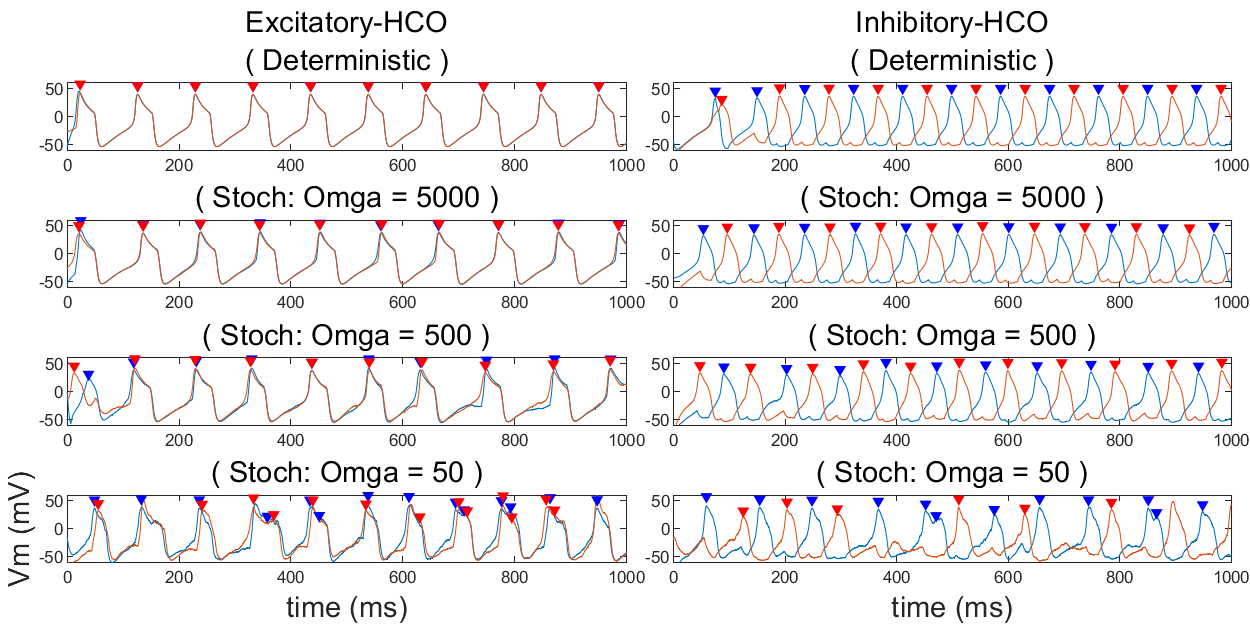
\includegraphics[width=\textwidth]{figs/F3_A_HCO_Omega_NB.png}
  \end{subfigure}
  \vspace{-0.5cm}
  \caption{(A) HCO with non-bursting ML neurons}
\end{figure}

Figure \ref{fig:fig3nb} shows HCO with plain ML neurons with inhibitory and excitatory synapses. Stimulus current is enabled for each of these neurons, \(I_{stim}=95\). Effect of noise level is seen through varying system size, (\(\Omega_{M,N}\)).

\hypertarget{bursting-mode-ml-neurons-hco}{%
\subsubsection{Bursting mode ML neurons HCO}\label{bursting-mode-ml-neurons-hco}}

\begin{figure}    \ContinuedFloat
  \captionsetup[subfigure]{labelformat=empty} \centering
  \begin{subfigure}[b]{\textwidth}
      \caption{} \label{fig:fig3b}
      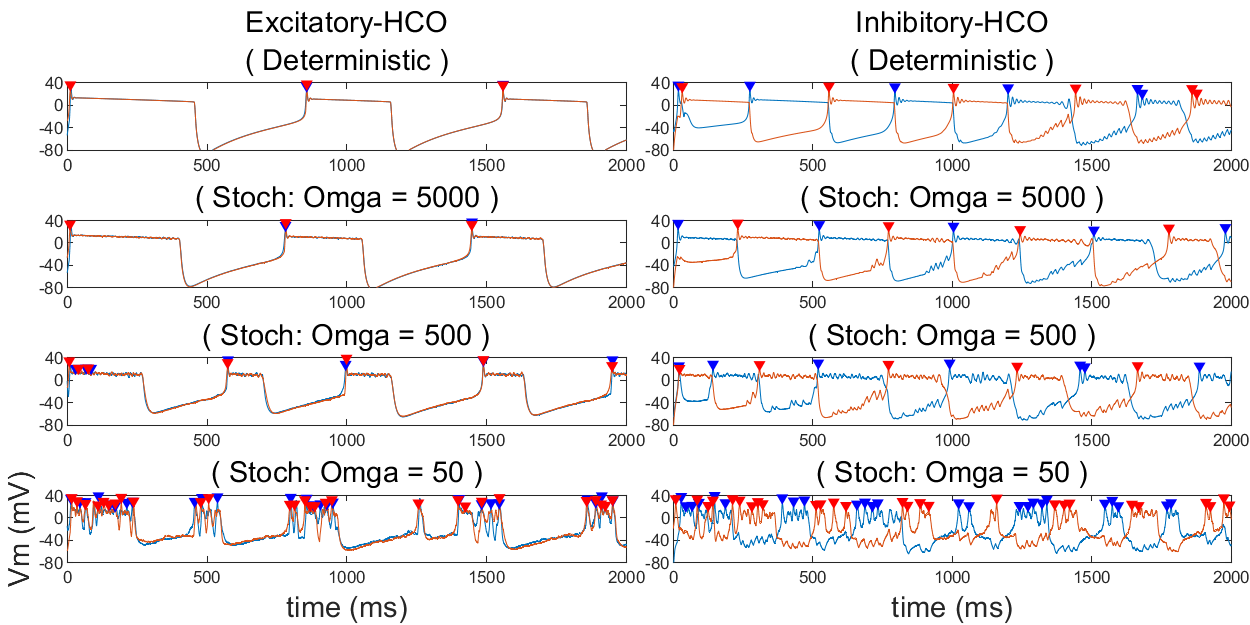
\includegraphics[width=\textwidth]{figs/F3_B_HCO_Omega_B.png}
  \end{subfigure}
  \vspace{-0.5cm}
  \caption{(B) HCO with bursting ML neurons}
\end{figure}

Similarly, HCO with bursting ML neurons is shown in Figure \ref{fig:fig3b} where stimulus current is set to zero and each neuron is having internal feedback current.

It appears that both excitatory and inhibitory HCOs show synchronization where the e-HCO show in-phase oscillations and i-HCO show out-phase oscillations. In general, lower noise level shows tight coupling between the oscillators in either case. (See section \ref{CD} for discussion).

\hypertarget{MLsync}{%
\subsection{Measuring Synchrony}\label{MLsync}}

Once I get the voltage traces of both the neurons, I measure the amount of synchronization for each HCO type, and later to compare the synchronization among all types. For measuring synchrony I use two methods.

\begin{enumerate}
\def\labelenumi{\arabic{enumi}.}
\tightlist
\item
  Cross-correlation of two raw voltage traces.
\item
  Gaussian smoothed spike-time based binless correlation.
\end{enumerate}

The first method does not make any assumptions and it compares raw voltage traces to each other to each other. Pearson's linear correlation coefficient is fond for the normalized voltage traces of neuron-1 and neuron-2 for a given HCO. However, this method can be influenced by the noise levels in the system, which can be an issue for lower system size simulations. So, in addition to this method, I am also using gaussian smoothed spike-train for finding correlation, which incurs less error than simple \emph{peristimulus time histogram} (PSTH) as this method uses gaussian kernel and eliminates the noise generated from binning of the spike times, as previously described in detail (Kruskal et al. 2007; Victor and Purpura 1997).

\hypertarget{spk}{%
\subsubsection{Detect spikes}\label{spk}}

\begin{figure}
  \centering
  \begin{subfigure}[b]{\textwidth}
    \centering
    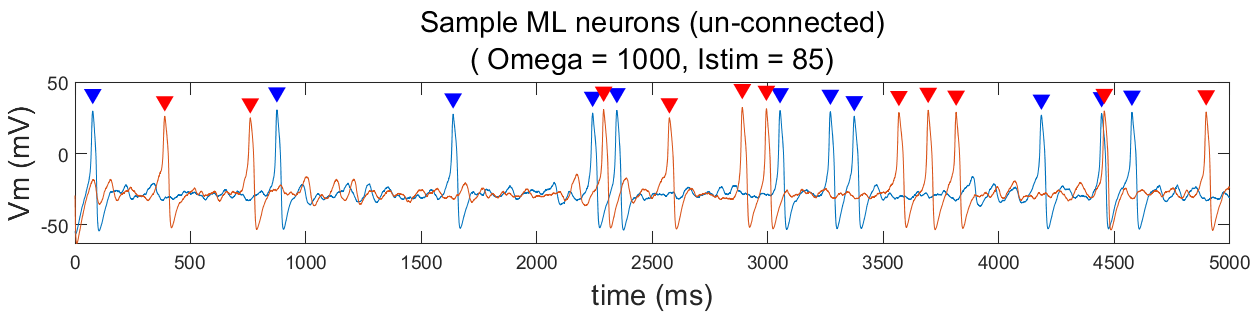
\includegraphics[width=\textwidth]{figs/F4_sample_ML.png}
  \end{subfigure}
  \vspace{-0.5cm}
  \caption{Detecting spikes in ML neurons using amplitude threshold of 15mV.}  \label{fig:fig4}
\end{figure}

I am finding and saving spike-times along with raw voltage traces for each simulation because one of the methods to quantify synchronization requires them. Figure \ref{fig:fig4} shows threshold based spikes detection result for a sample ML neuron with the voltage threshold set to 15 mV. I find local maxima to identify peaks in a signal. I use a refractory period of 15ms to avoid detecting multiple spikes for a single action potential, which would have been an issue when an unfiltered neuron has multiple local-maxima. Two sample neurons here are not connected to each other via any synapse.

\hypertarget{blc}{%
\subsubsection{Gaussian smoothing}\label{blc}}

\begin{figure}
  \centering
  \begin{subfigure}[b]{\textwidth}
      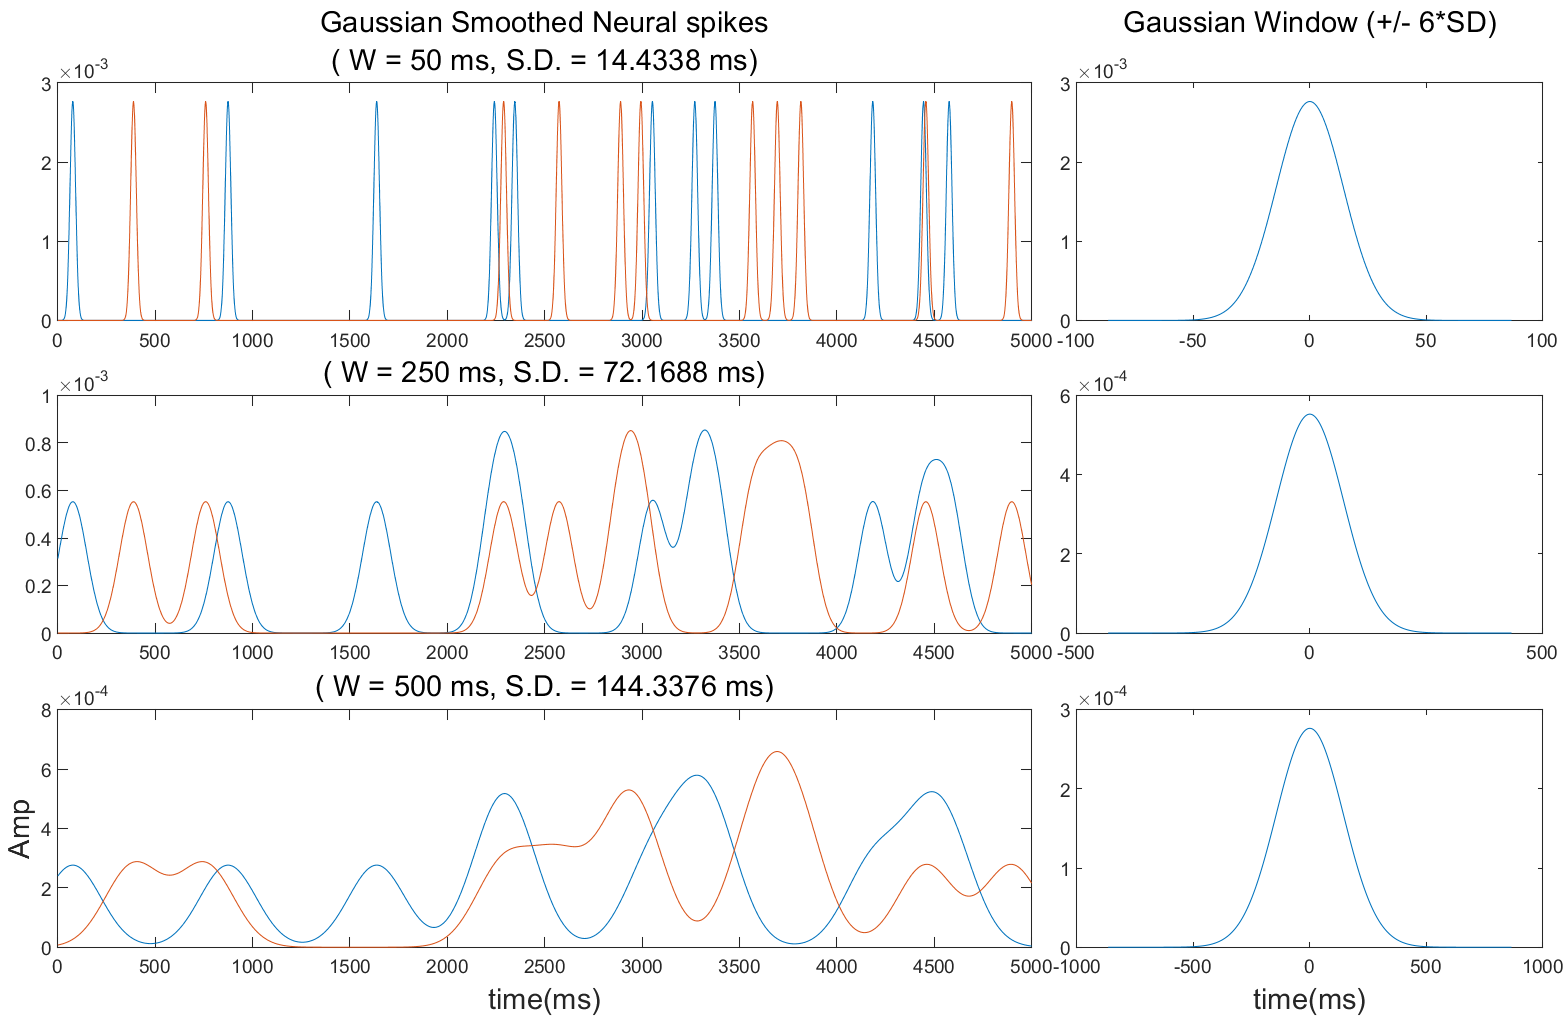
\includegraphics[width=\textwidth]{figs/F5_GCFR_GW.png}
  \end{subfigure}
  \vspace{-0.5cm}
  \caption{Gaussian smoothing of spike trains with Gaussian kernel of different $\sigma$.} \label{fig:fig5gcfr}
\end{figure}

Previously Figure \ref{fig:fig4} shows identified spike-times (filled markers) and raw membrane voltage traces for two ML neurons. Here, in the Figure \ref{fig:fig5gcfr} the gaussian-smoothed spike-train with a gaussian-kernel of different \(\sigma\) (S.D.) are shown for the same neurons 1 and 2. Gaussian window size calculated from the Bin-Width (\(W\)) using \(\sigma=W/\sqrt12\) (Kruskal et al. 2007). Kernels are shown in the figure on the right pane.

\hypertarget{single-run-effect-of-bin-width-on-cross-correlation}{%
\subsubsection{Single Run : Effect of bin-width on cross-correlation}\label{single-run-effect-of-bin-width-on-cross-correlation}}

As previously shown, varying \(\sigma\) would change the gaussian-smoothed spike trains, and subsequently it will change the correlation. Here I am comparing correlation coefficient found for various bin-width (thus, varied \(\sigma\)) and comparing it across a wider range of noise levels (i.e., \(\Omega_{M,N}=\{5e4, 5e3, 5e2, 5e1, 5e0\}\)) for each HCO types.

\begin{figure}
  \centering
  \begin{subfigure}[b]{0.75\textwidth}
      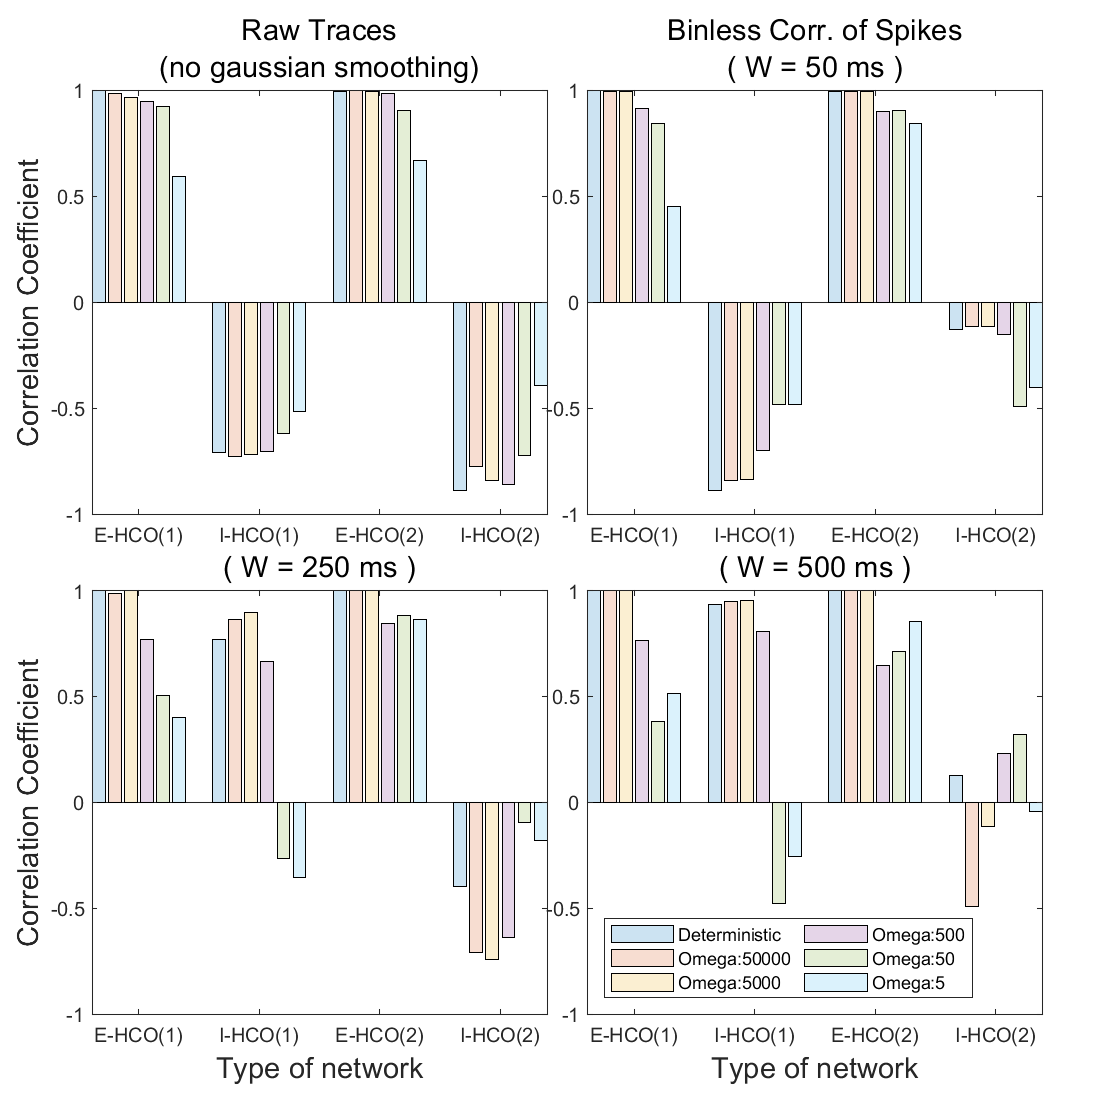
\includegraphics[width=\textwidth]{figs/F6_HCO_corr_single_run.png}
  \end{subfigure}
  \vspace{-0.25cm}
  \caption{Single iteration values of spike train correlation for various kinds of HCOs and for different system sizes.} \label{fig:fig6}
\end{figure}

Figure \ref{fig:fig6} shows correlation of raw traces (i.e., without identifying spike-times) in upper left corner; and also shows the effect of S.D. of the gaussian window (i.e., \(\sigma=W/\sqrt12\)) used for getting the binless correlation between the spike trains. The raw membrane voltage traces for each of the neurons in all the HCOs are shown in Appendix, Figure-\ref{fig:figx1}. It is apparent that raw traces and smaller bin-width (W=50) yields more similar correlation than the higher bin-widths (W=250,500) and increasing the noise levels generally reduces the coupling of the oscillators. Wider bin-width shows higher value of correlation as compared to smaller widths. (See section \ref{CD} for discussion).

\hypertarget{results}{%
\section{Results}\label{results}}

While finding such correlation I noticed that some values were fluctuating a lot across the trials, thus, I was getting slightly varying plots of Figure \ref{fig:fig6}. So, for comparing the effect of noise (i.e., system size) on various kinds of HCOs, I plotted the correlations of multiple iterations (n=25) on a semi-log scale plot. The result is shown in Figure \ref{fig:fig7}.

\begin{figure}
  \centering
  \begin{subfigure}[b]{\textwidth}
    \centering
    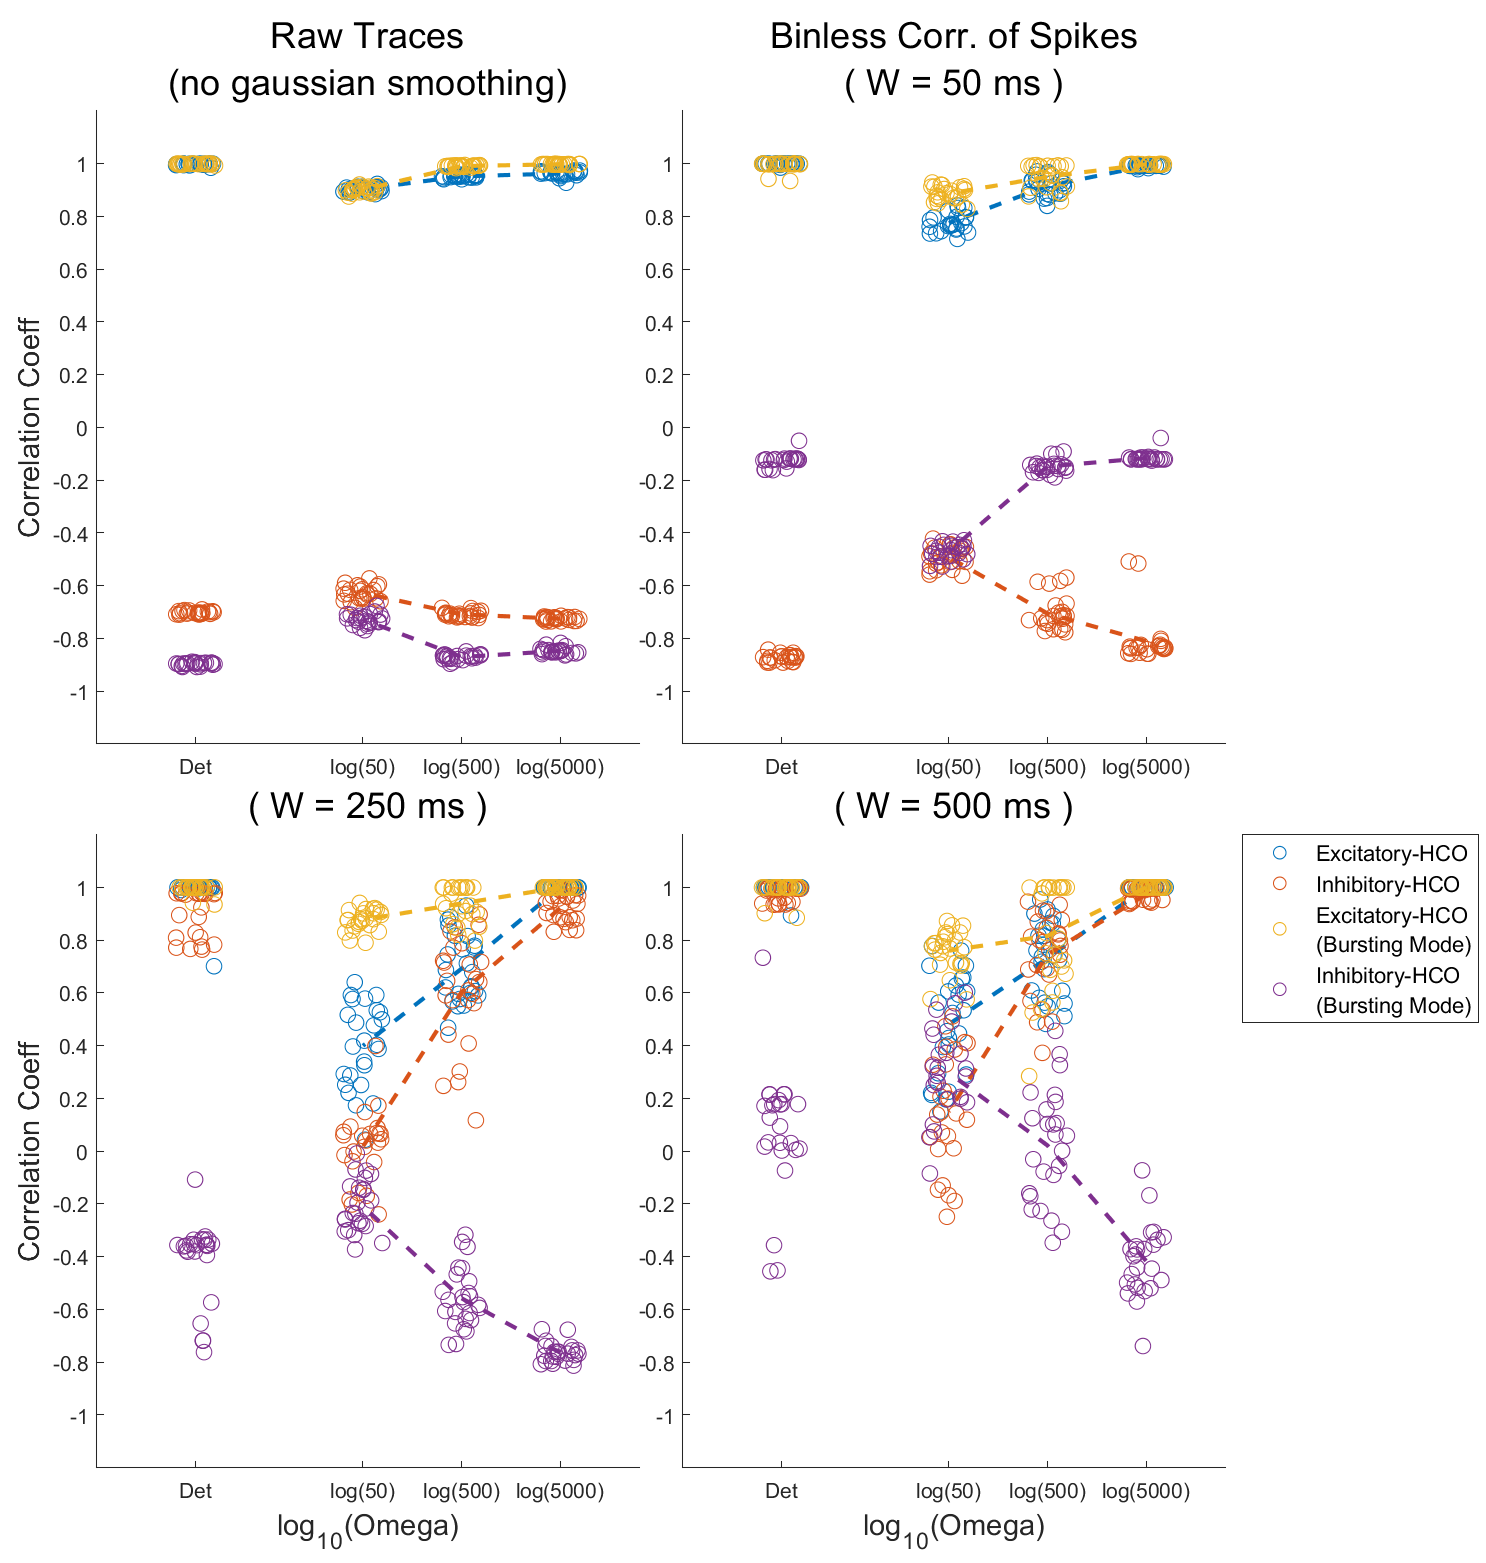
\includegraphics[width=\textwidth]{figs/F7_HCO_BLCorr_omega.png}
  \end{subfigure}
  \vspace{-0.5cm}
  \caption{Comparing binless correlations in different types of HCOs for multiple runs (n=25).}  \label{fig:fig7}
\end{figure}

(Note : Correlation values in the scatterplot in Figure \ref{fig:fig7} contain a small jitter in X-axis direction, to better visualize the points and variabilities without affecting their Y-axis values.)

Figure \ref{fig:fig7} quantifies the synchronization between two neuron cells simulated using deterministic and stochastic methods while varying noise levels. The correlation values are compared across different methods of finding correlation (i.e., raw traces without gaussian smoothing and with gaussian smoothing using various kernel sizes). Smaller kernel (W=50) gives less variable results across multiple iterations. Positive values show in-phase synchronization and negative values here suggest out-of phase synchronization. The absolute value suggests the strength of the coupling between neurons in the HCO. Following the raw traces and binless correlation (W=50), it is apparent that reducing noise levels (i.e, higher \(log_{10}(\Omega\)) values) give stronger correlation of the oscillators and deterministic simulation gives similar results with small noise levels, as one would expect. More discussion on variabilities due to bin-width and counter-intuitive trends seen in bursting type inhibitory-HCO (in purple) is done in the following section (See Section \ref{CD}).

\hypertarget{CD}{%
\section{Discussion and Conclusions}\label{CD}}

\begin{enumerate}
\def\labelenumi{\arabic{enumi}.}
\tightlist
\item
  \textbf{Higher binwidth in binless correlation leads to more variabilities and inflated correlation values.}
\end{enumerate}

Figure \ref{fig:fig7} shows correlation comparison for different HCOs computed using various methods in 25 iterations. Firstly, variations of the values across 25 iterations are more when the gaussian kernel used is wider (e.g., W=250, 500, etc.) and also with this method, more values show positive correlation as compared to negative correlation. This may be the case because wider kernels would overlap more for neighboring spikes and show an overall positive (i.e., in phase) correlation as opposed to anti-phased correlation. Higher variabilities indicate that gaussian smoothing using a larger gaussian kernel would make correlation coefficient more sensitive for the relative spike position. For example, if there are more than one spike present close-by, this method would give very high signal for them (see in Figure \ref{fig:fig5gcfr}), and ultimately this becomes an issue as the gaussian smoothed signal would vary quite a lot based on randomness in spike position.

\begin{enumerate}
\def\labelenumi{\arabic{enumi}.}
\setcounter{enumi}{1}
\tightlist
\item
  \textbf{Binless correlation (with small width kernel) is more efficient in predicting correlation for non-bursting HCOs and excitatory-HCOs.}
\end{enumerate}

While comparing raw traces and 50ms window results, one can see that gaussian smoothing works better for non-bursting type HCOs (in blue, yellow). That is because raw correlation depends on the actual shape of the spikes (see Figure \ref{fig:fig3nb}) and binless correlation only uses identified spike-times. So, with higher noise in simulation (i.e., low omega), a spike in one neuron may fail to cause a spike in another neuron, yet the shape of the raw trace would change which may lead the raw-signal method to count higher higher correlation than spike-time based method. Also due to noise levels, if the peaks are not aligned but the overall spike shapes are matching, the same thing may happen. Thus, here binless correlation with identified spike-times is more useful for predicting correlation given certain noise levels.

\begin{enumerate}
\def\labelenumi{\arabic{enumi}.}
\setcounter{enumi}{2}
\tightlist
\item
  \textbf{For bursting type inhibitory-HCO binless correlation with ``wider-width'' kernels works the best. Binless correlation with small-width kernel is in-efficient and raw-traces method completely disregard spike-times in favor of slow \emph{plateau potential}.}
\end{enumerate}

See bursting inhibitory-HCO (in Purple) in Figure \ref{fig:fig7}, for which the trend looks very different between raw-traces and 50ms kernel methods. This is mainly because the raw-traces method would largely influenced by the \emph{plateau potential} due to slow internal bursting current, whereas in the binless correlation method the only identified spike-times would be used due to the pattern our bursting-ML neurons use, the fast current feedback (i.e., a spike) would vary a lot based on the coupling type and noise level. Thus, the binless method shows it more like un-synchronized (i.e., values close to zero) for inhibitory HCOs and raw-traces method show it as anti-phased synchronized, the result largely driven by the slow \emph{plateau potentials}.

However, a wider-width kernel would disregard the exact spike-times but still works better for inhibitory-bursting-HCOs (see W=250, Figure \ref{fig:fig7}). This is because the \emph{plateau potentials} itself oscillates (i.e., turns on-and-off) and the spikes are segregated in chunks (see \ref{fig:fig3b}), so the gaussian smoothed traces with wider kernels would also oscillate in anti-phase. So, one can see why the wider-kernel is more efficient in predicting correlation for bursting type inhibitory-HCOs.

\begin{enumerate}
\def\labelenumi{\arabic{enumi}.}
\setcounter{enumi}{3}
\tightlist
\item
  \textbf{Simple oscillator made using two ML neurons shows synchronized oscillations.}
\end{enumerate}

At the very least, the simple altered ML neurons show synchronous firing when coupled through any type of synapse, creating a simple oscillator. Excitatory-HCOs show stronger correlations as compared to inhibitory-HCOs. For a sustained firing, and in-turn, achieve synchrony, ML neurons either need slow internal feedback current or constant external stimulus current.

\begin{enumerate}
\def\labelenumi{\arabic{enumi}.}
\setcounter{enumi}{4}
\tightlist
\item
  \textbf{Excitatory-HCOs show in-phase synchronization and inhibitory-HCOs show ant-phase synchronization. Reducing Noise improves the degree of synchrony.}
\end{enumerate}

As explained earlier in discussion points 2 and 3, synchronization for non-bursting-HCOs and excitatory-bursting-HCOs should be compared using binless correlation method with 50ms kernel (upper right, Figure \ref{fig:fig7})) and for bursting type inhibitory-HCO, I would use 250ms kernel (lower left, Figure \ref{fig:fig7})). Comparing the correlation coefficients, qualitatively, across various HCOs it appears that excitatory-HCOs (bursting and non bursting alike) show in-phase correlation, with bursting type HCO being higher tolerant to system noise levels. Similarly, inhibitory-HCOs show anti-phase synchronization.

\clearpage

\hypertarget{appendix-appendix}{%
\appendix}


\hypertarget{appendix-a-single-run-raw-plots-omega-and-hco-types}{%
\section{\texorpdfstring{Appendix A : Single-Run Raw Plots (\(\Omega\) and HCO types)}{Appendix A : Single-Run Raw Plots (\textbackslash Omega and HCO types)}}\label{appendix-a-single-run-raw-plots-omega-and-hco-types}}

These plots are the raw voltage traces for each neurons in all HCOs, which are used to compute single run correlations in Figure \ref{fig:fig6}.

\begin{figure}
  \centering
  \begin{subfigure}[b]{\textwidth}
    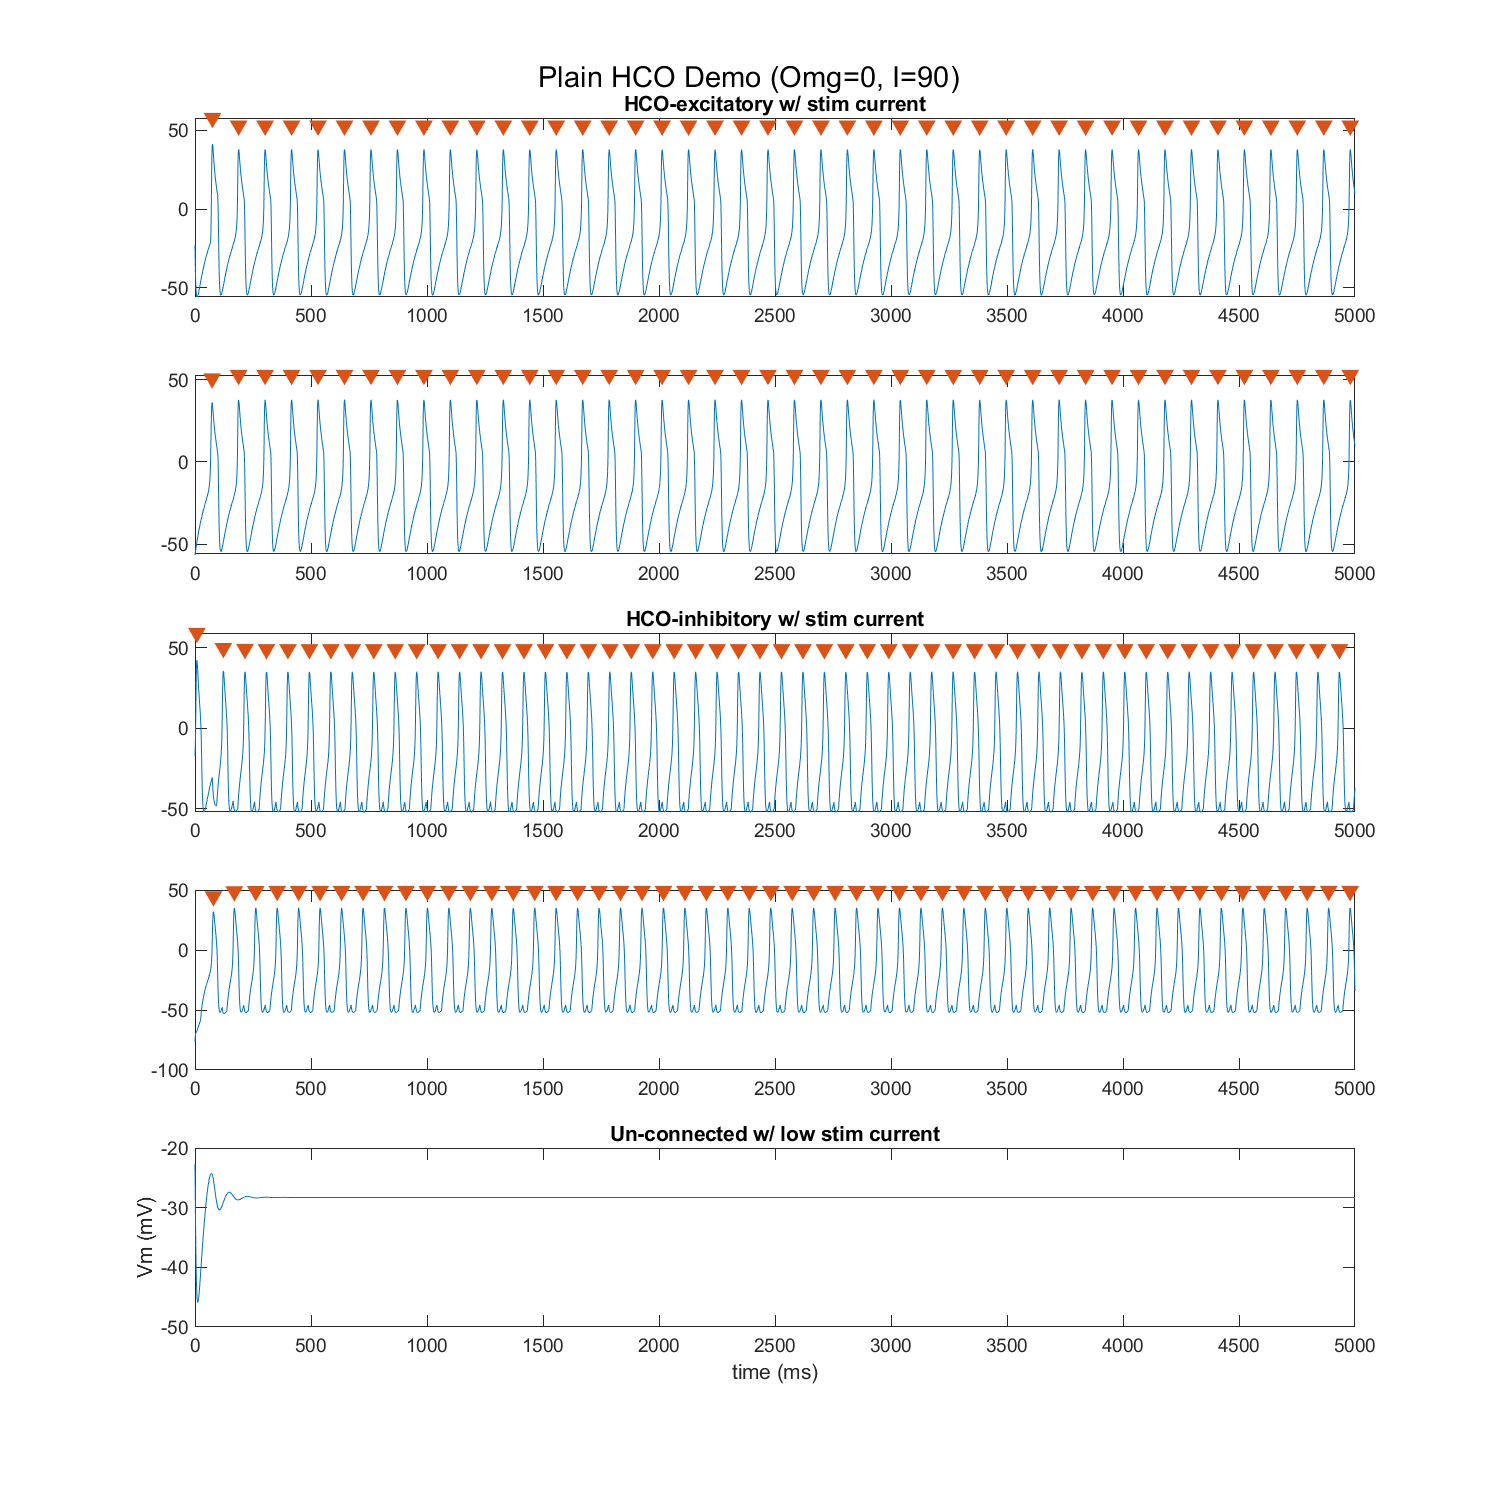
\includegraphics[width=.49\textwidth]{figs/old/Fx1_A_det_NB.png}
    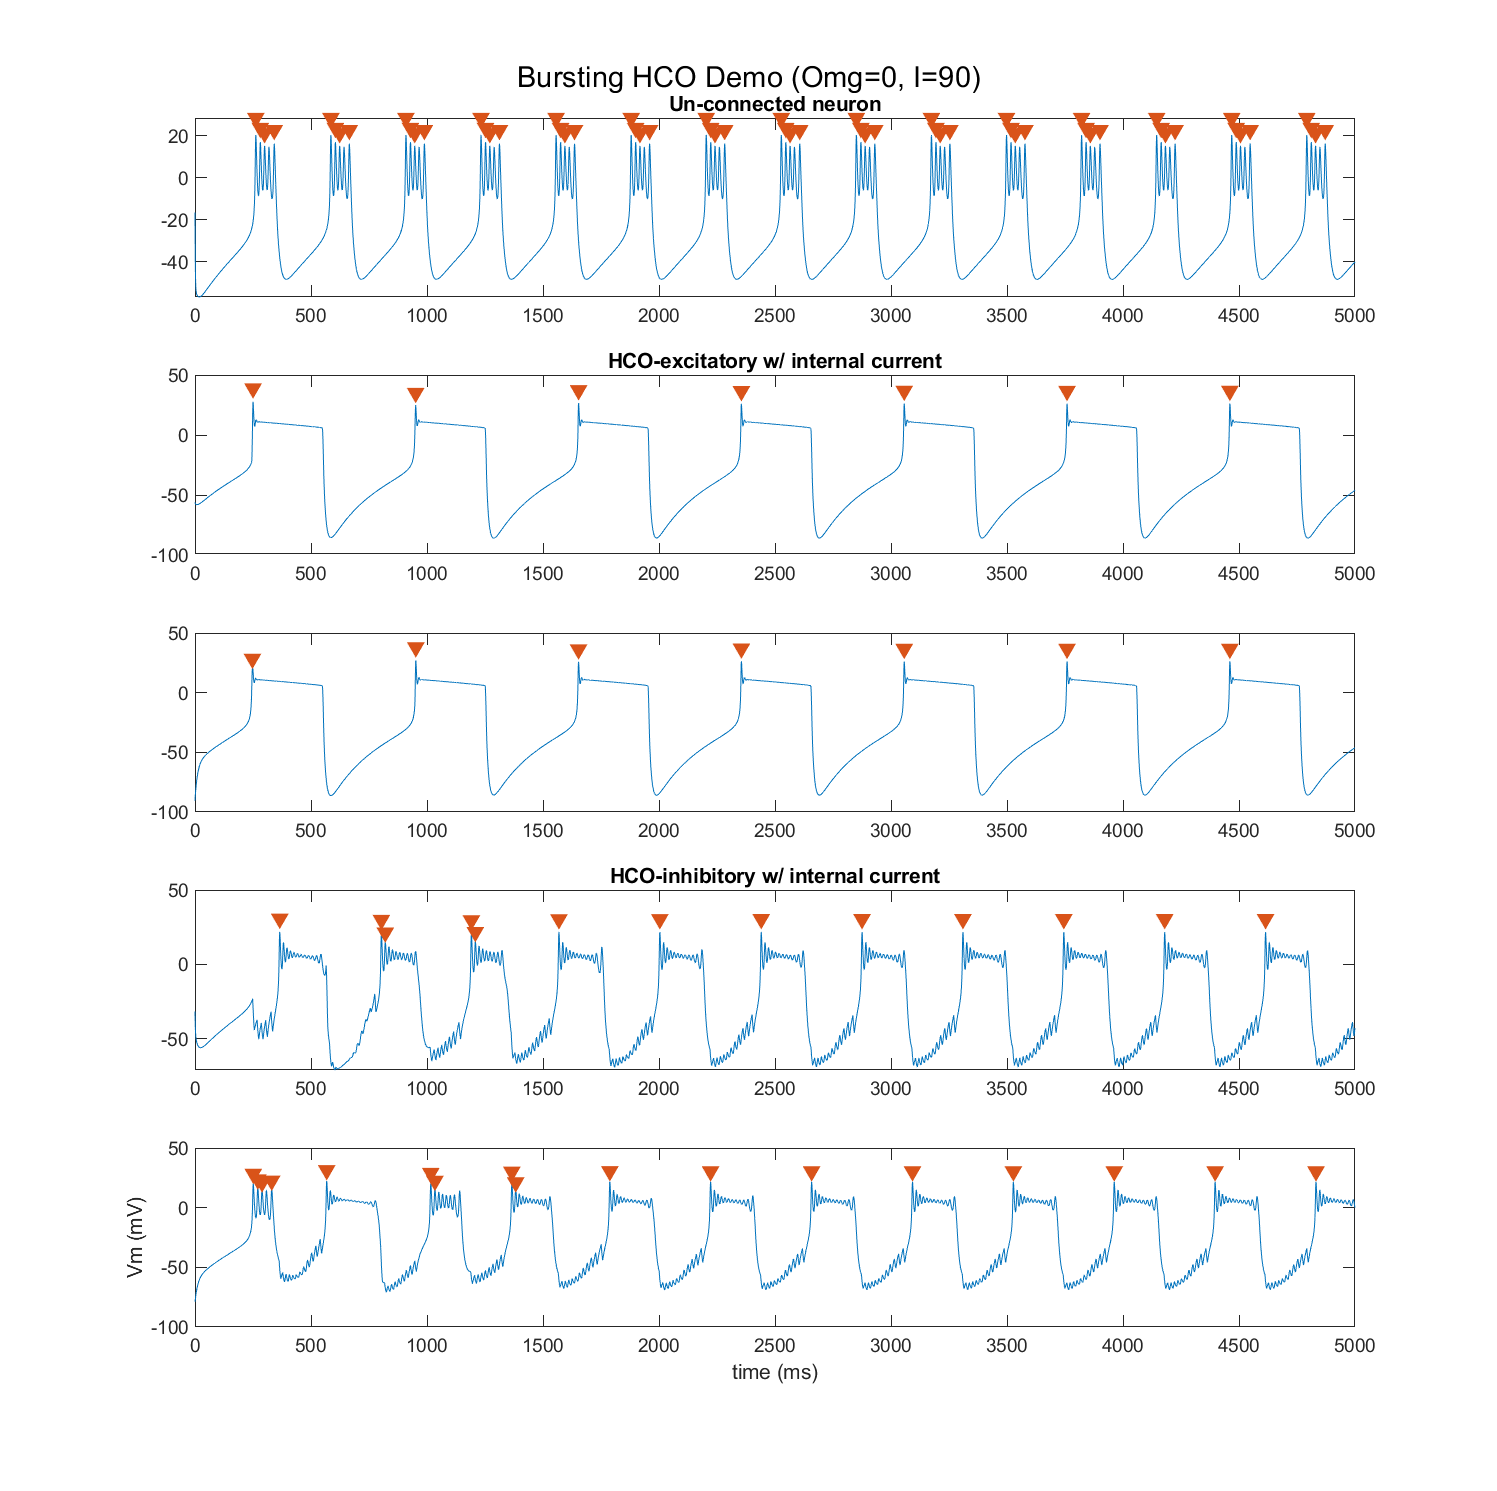
\includegraphics[width=.49\textwidth]{figs/old/Fx1_A_HCO_det_B.png}
    \vspace{-0.5cm} \caption{Deterministic HCO}
  \end{subfigure}
\end{figure}

\begin{figure} \ContinuedFloat
  \centering
  \begin{subfigure}[b]{\textwidth}  
    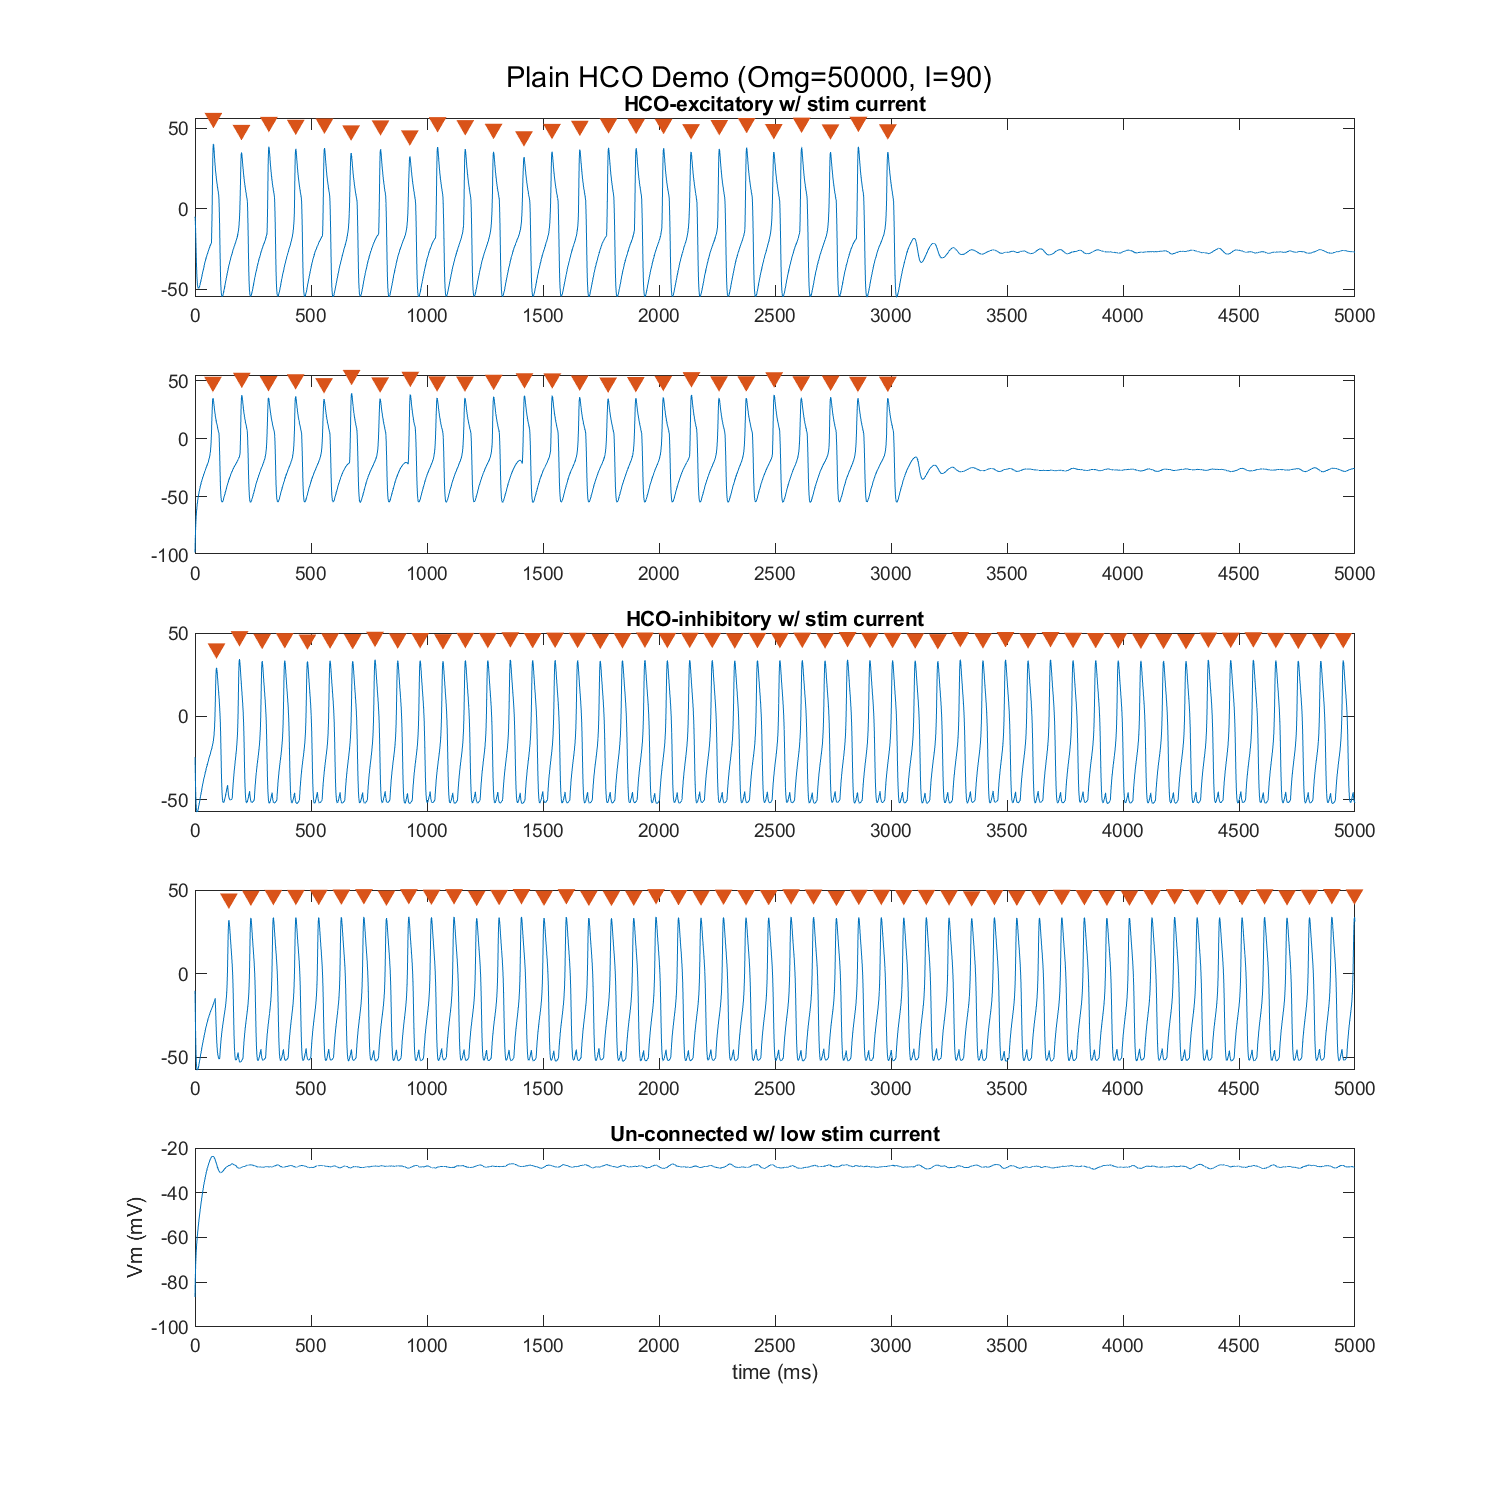
\includegraphics[width=.49\textwidth]{figs/old/Fx1_B_HCO_Om5e4_NB.png}
    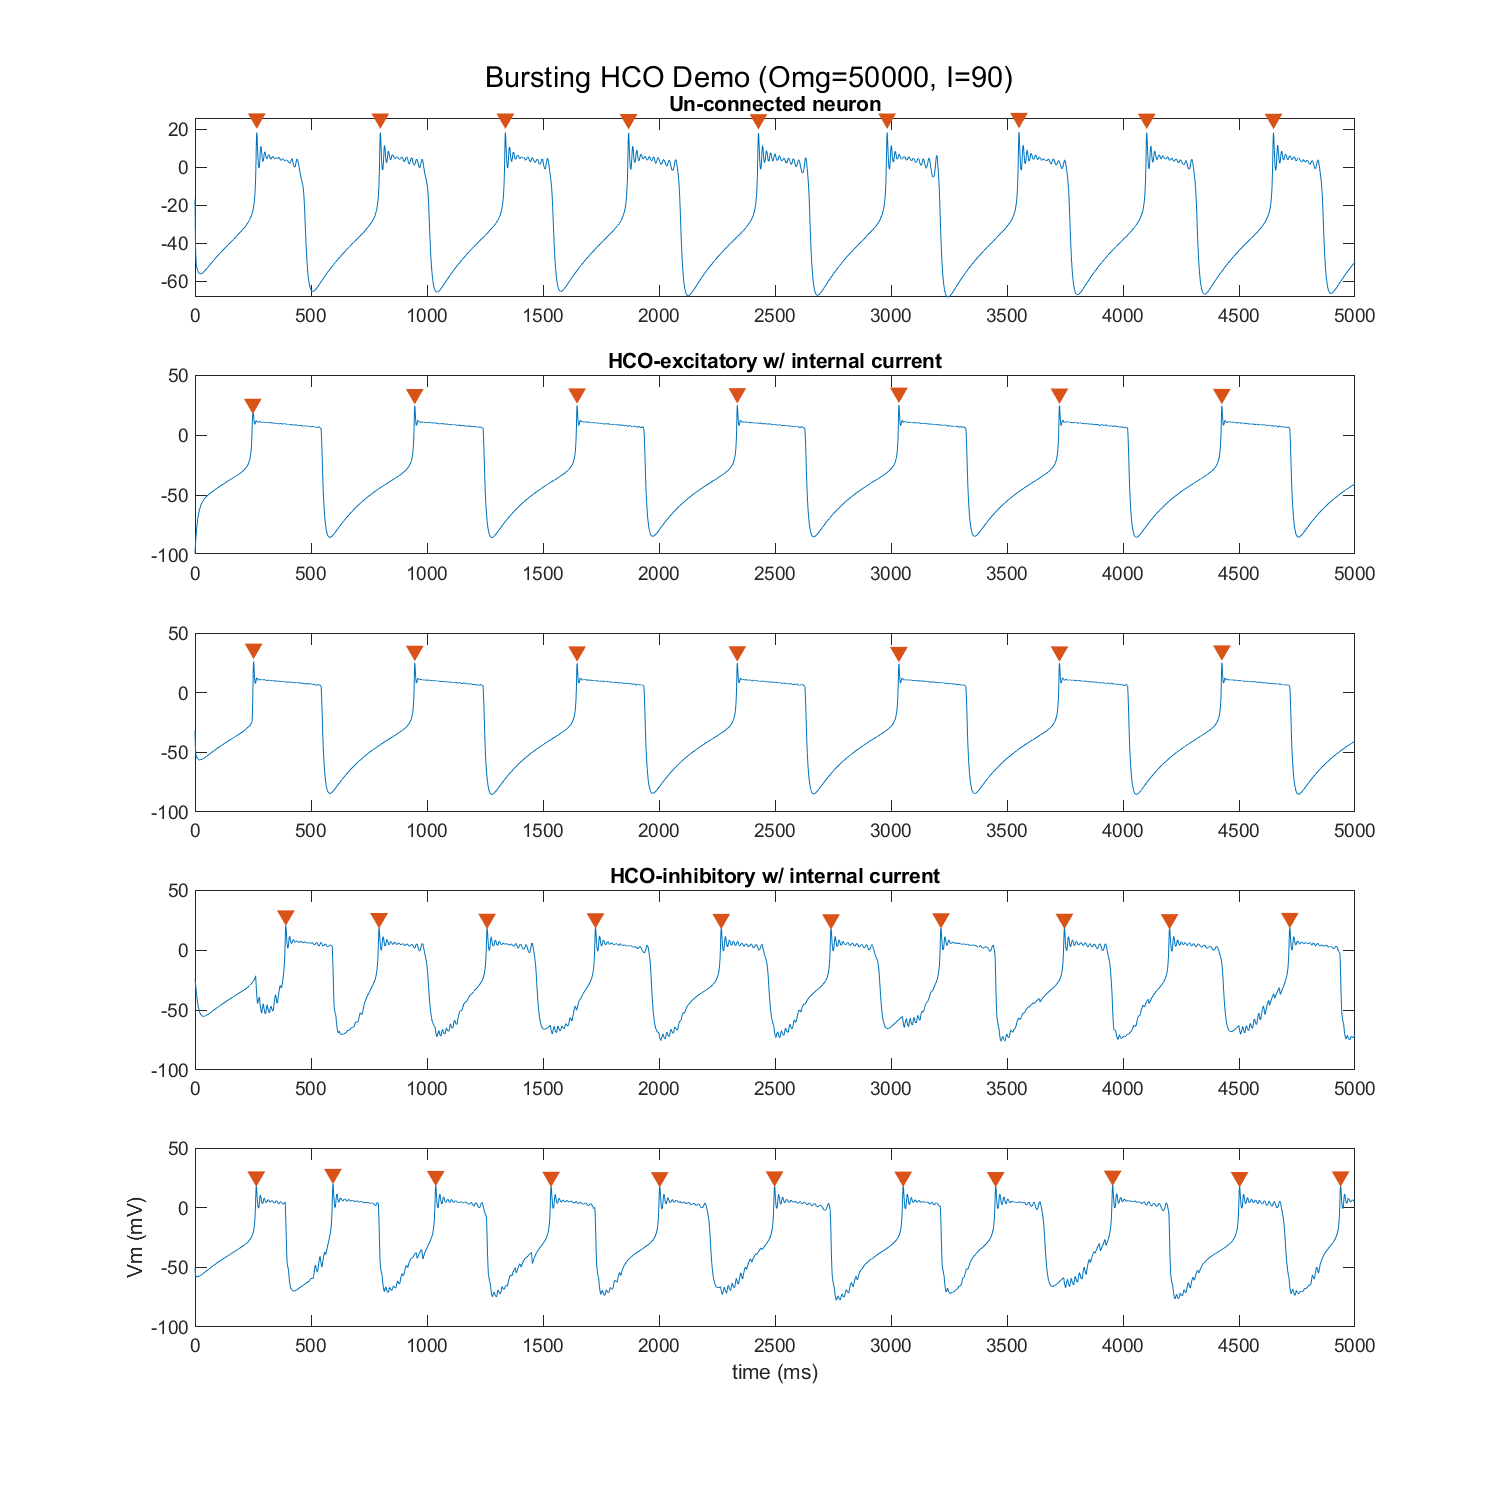
\includegraphics[width=.49\textwidth]{figs/old/Fx1_B_HCO_Om5e4_B.png}
    \vspace{-0.5cm} \caption{Stochastic HCO with Omega=50,000.}
  \end{subfigure}
\end{figure}

\begin{figure} \ContinuedFloat
  \centering
  \begin{subfigure}[b]{\textwidth}  
    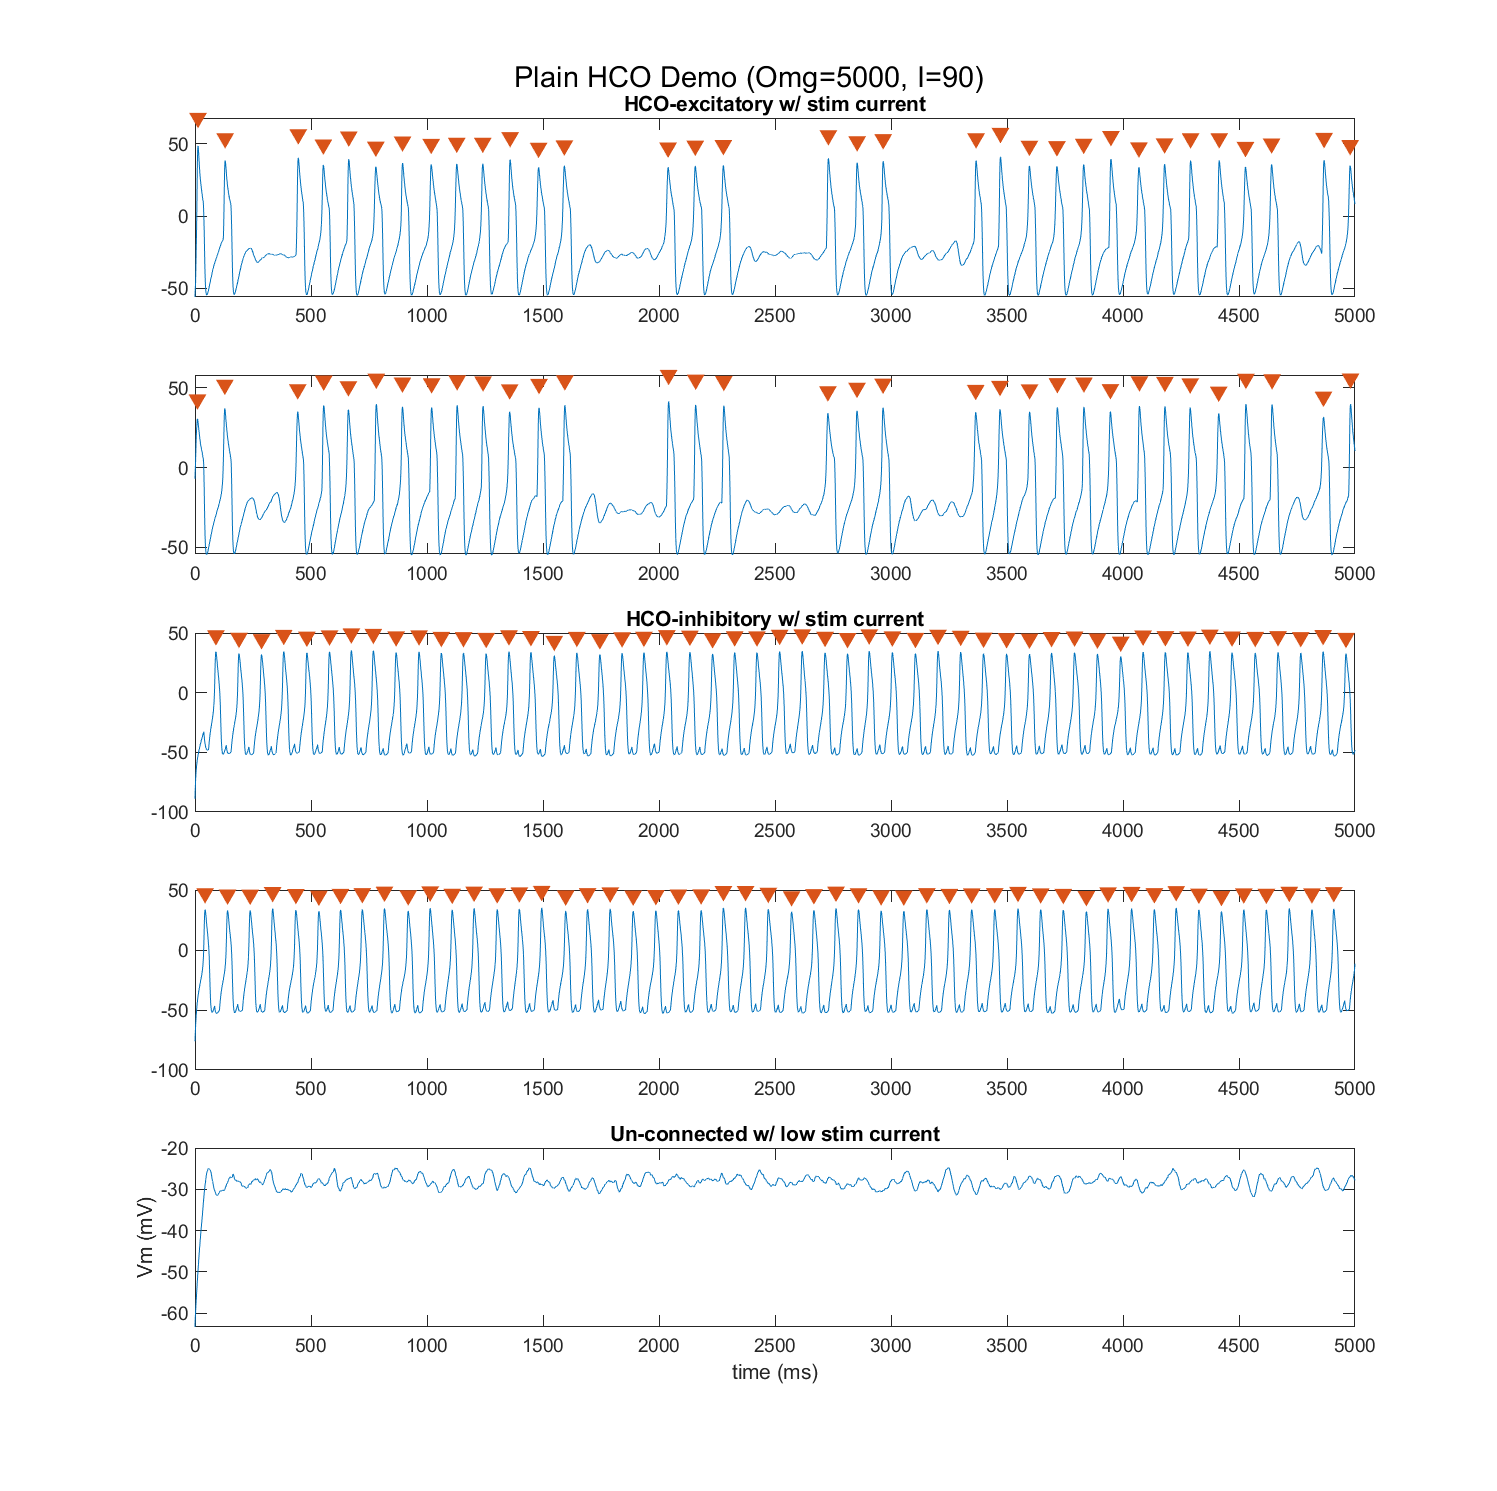
\includegraphics[width=.49\textwidth]{figs/old/Fx1_C_HCO_Om5e3_NB.png}
    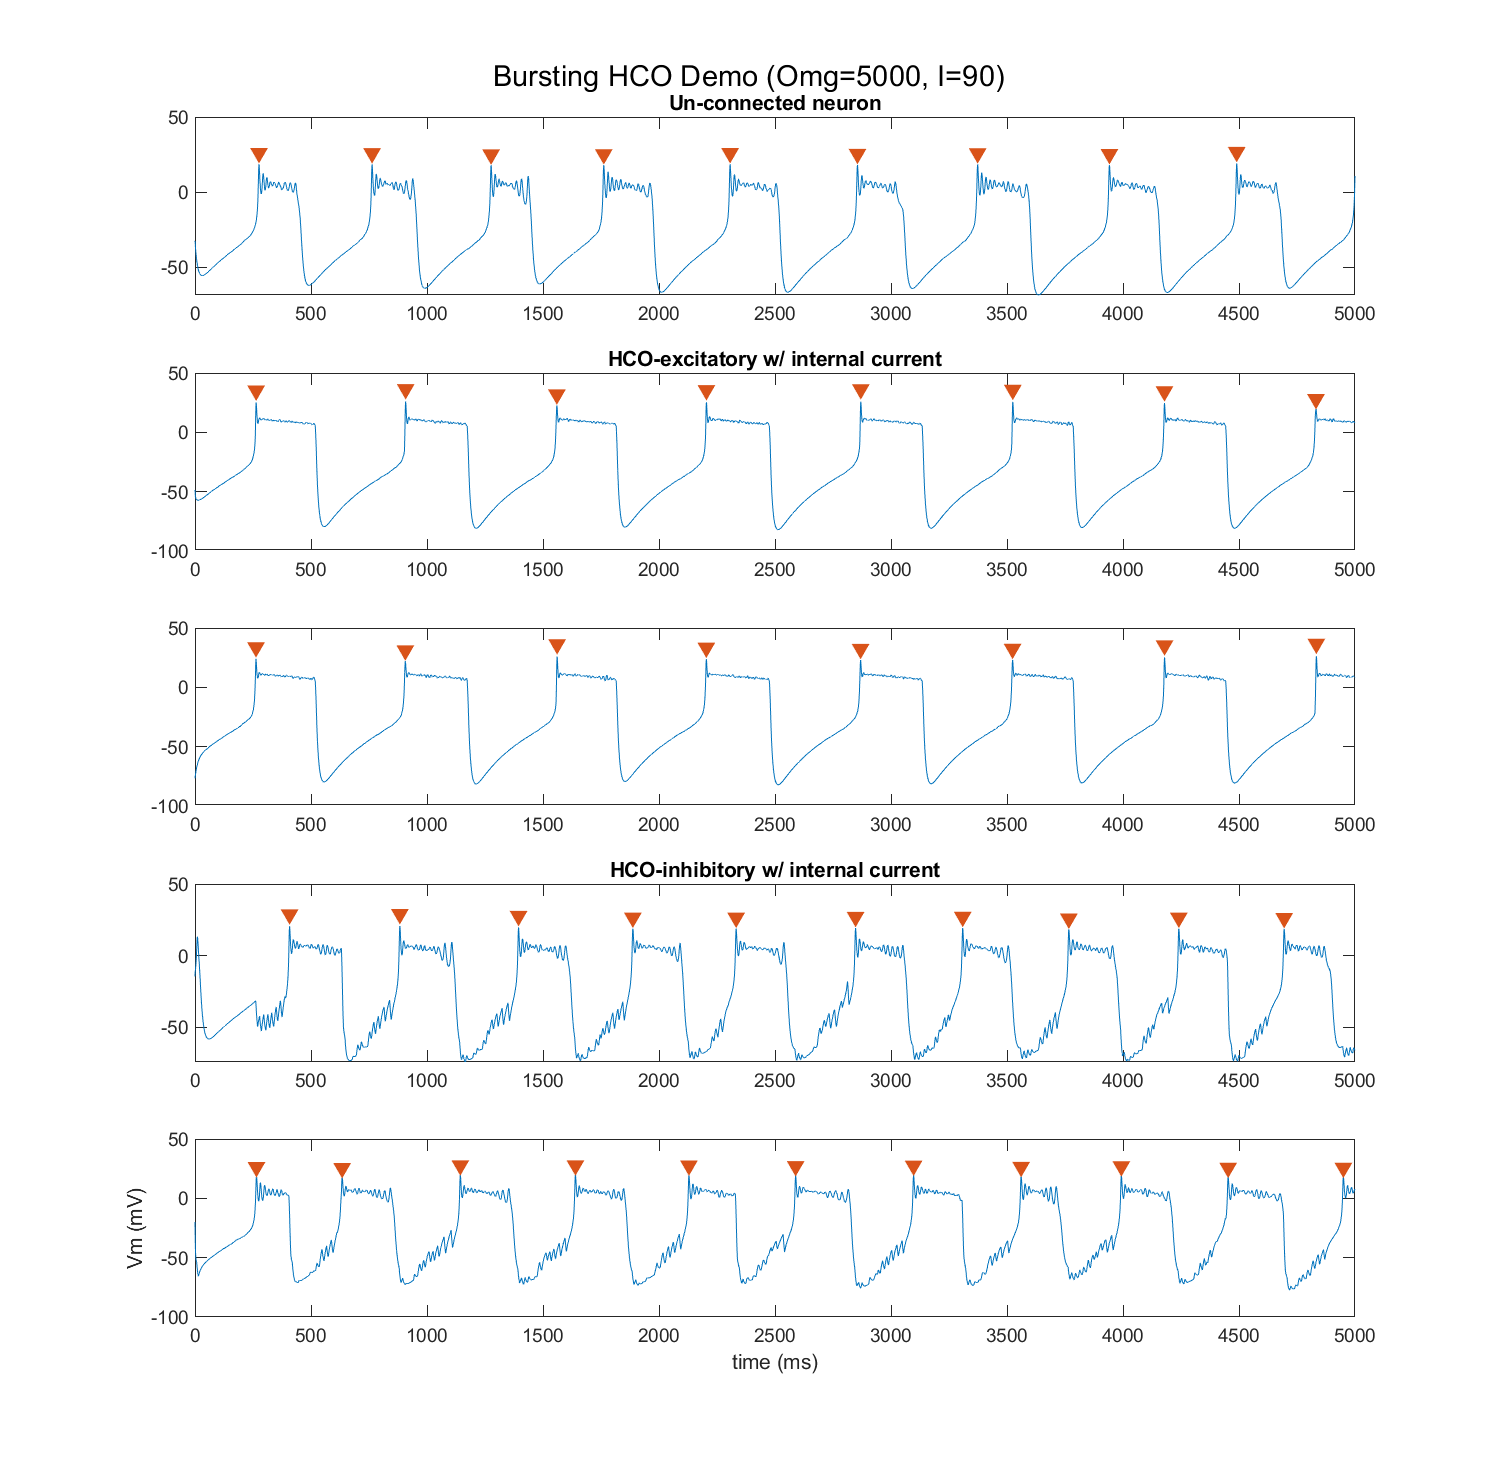
\includegraphics[width=.49\textwidth]{figs/old/Fx1_C_HCO_Om5e3_B.png}
    \vspace{-0.5cm} \caption{Stochastic HCO with Omega=5000.}
  \end{subfigure}
 \end{figure}

\begin{figure} \ContinuedFloat
  \centering
  \begin{subfigure}[b]{\textwidth}
    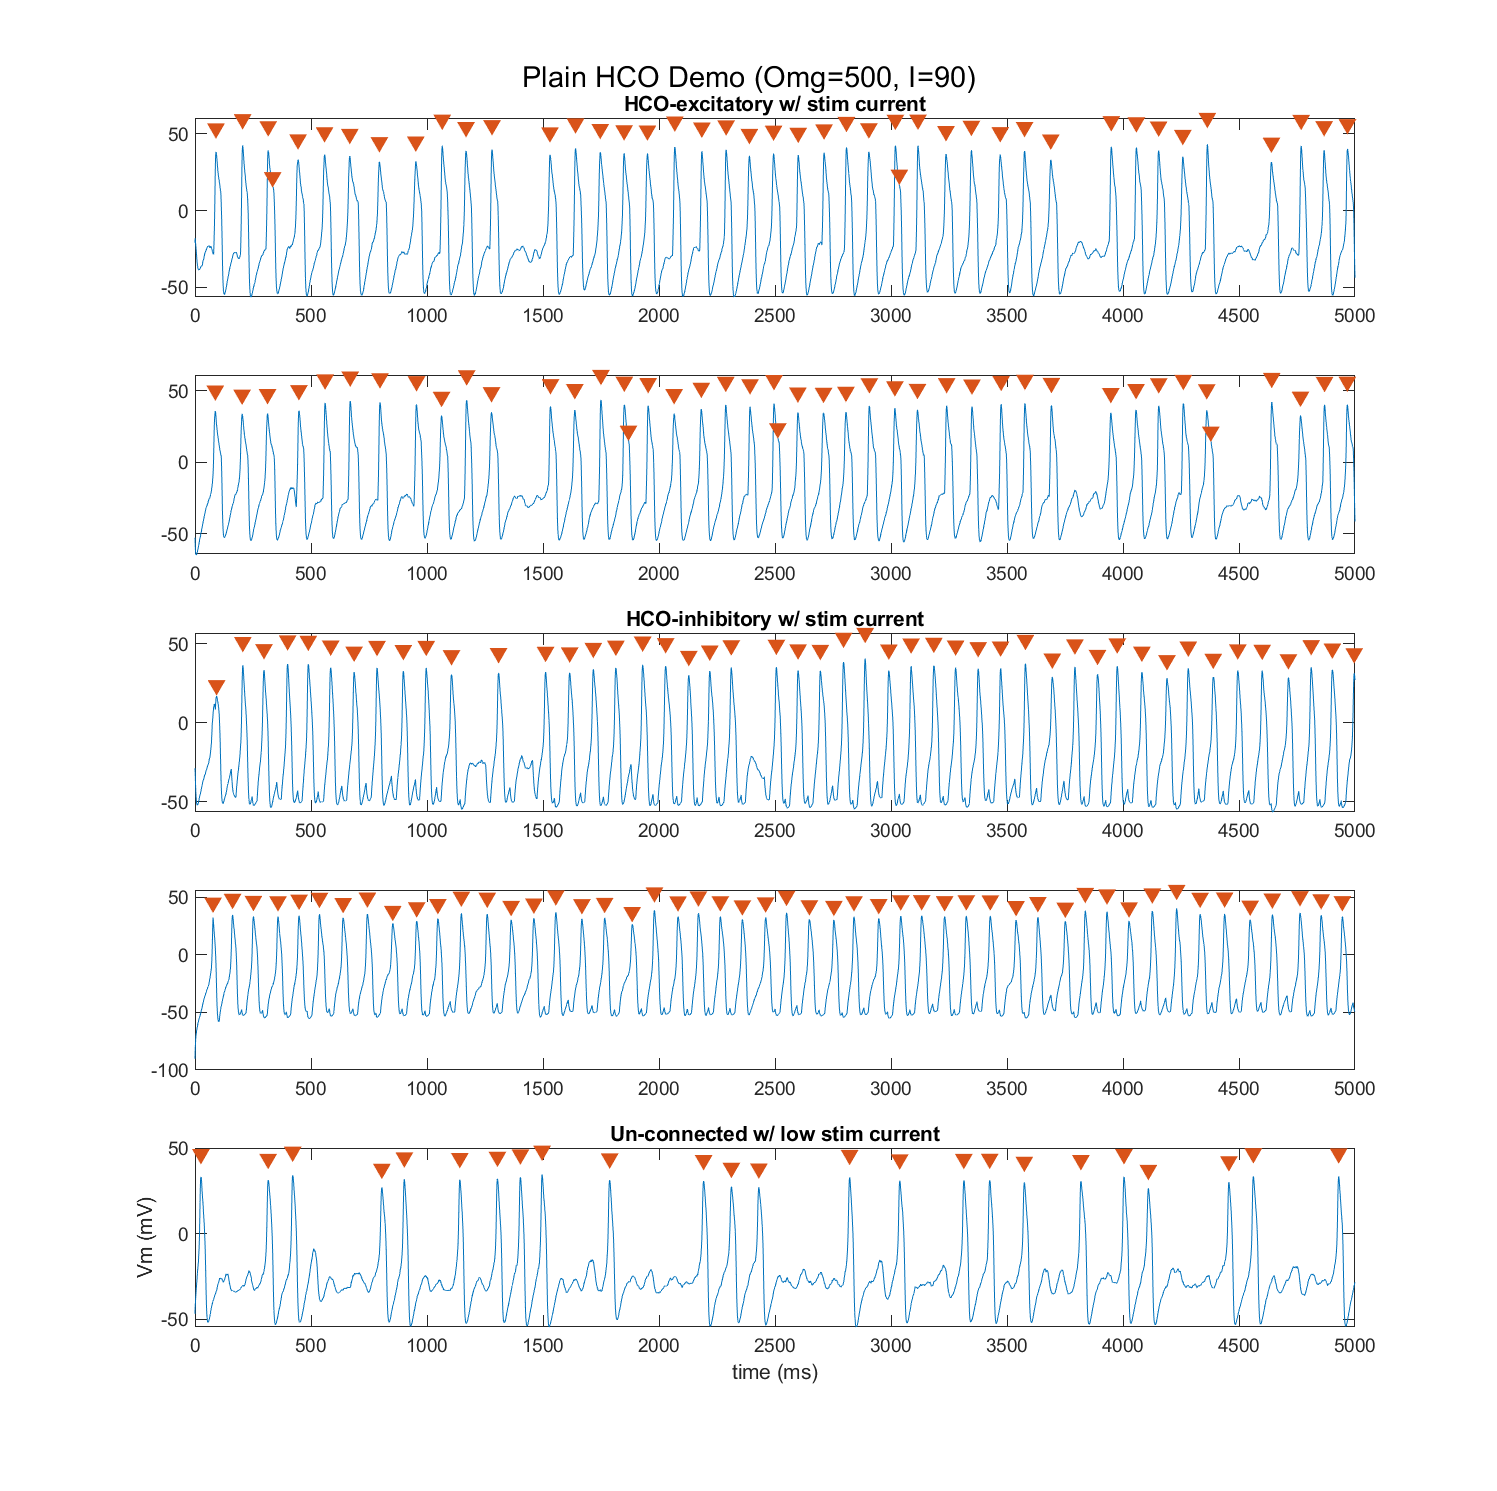
\includegraphics[width=.49\textwidth]{figs/old/Fx1_D_HCO_Om5e2_NB.png}         
    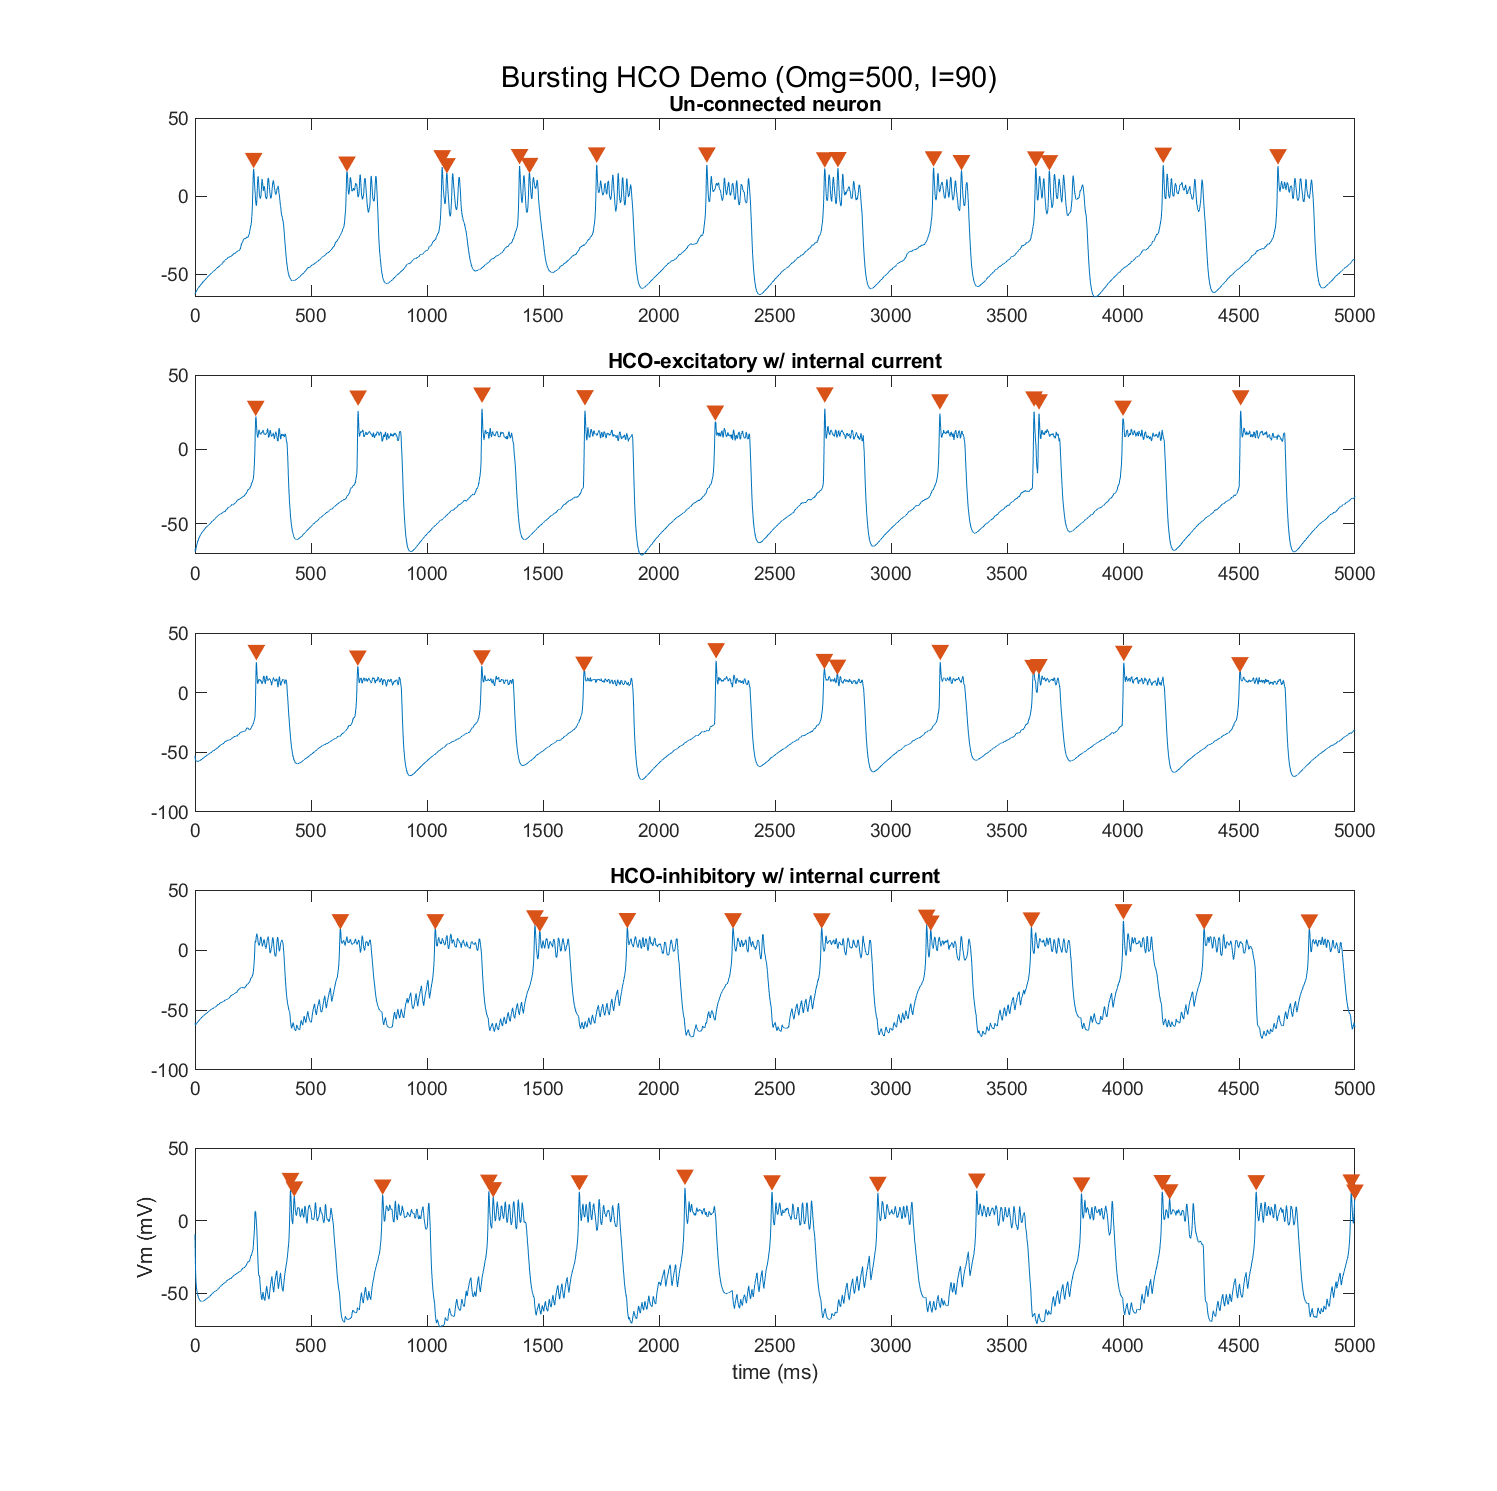
\includegraphics[width=.49\textwidth]{figs/old/Fx1_D_HCO_Om5e2_B.png}
    \vspace{-0.5cm} \caption{Stochastic HCO with Omega=500.}
  \end{subfigure}
\end{figure}

\begin{figure} \ContinuedFloat
  \centering
  \begin{subfigure}[b]{\textwidth}  
    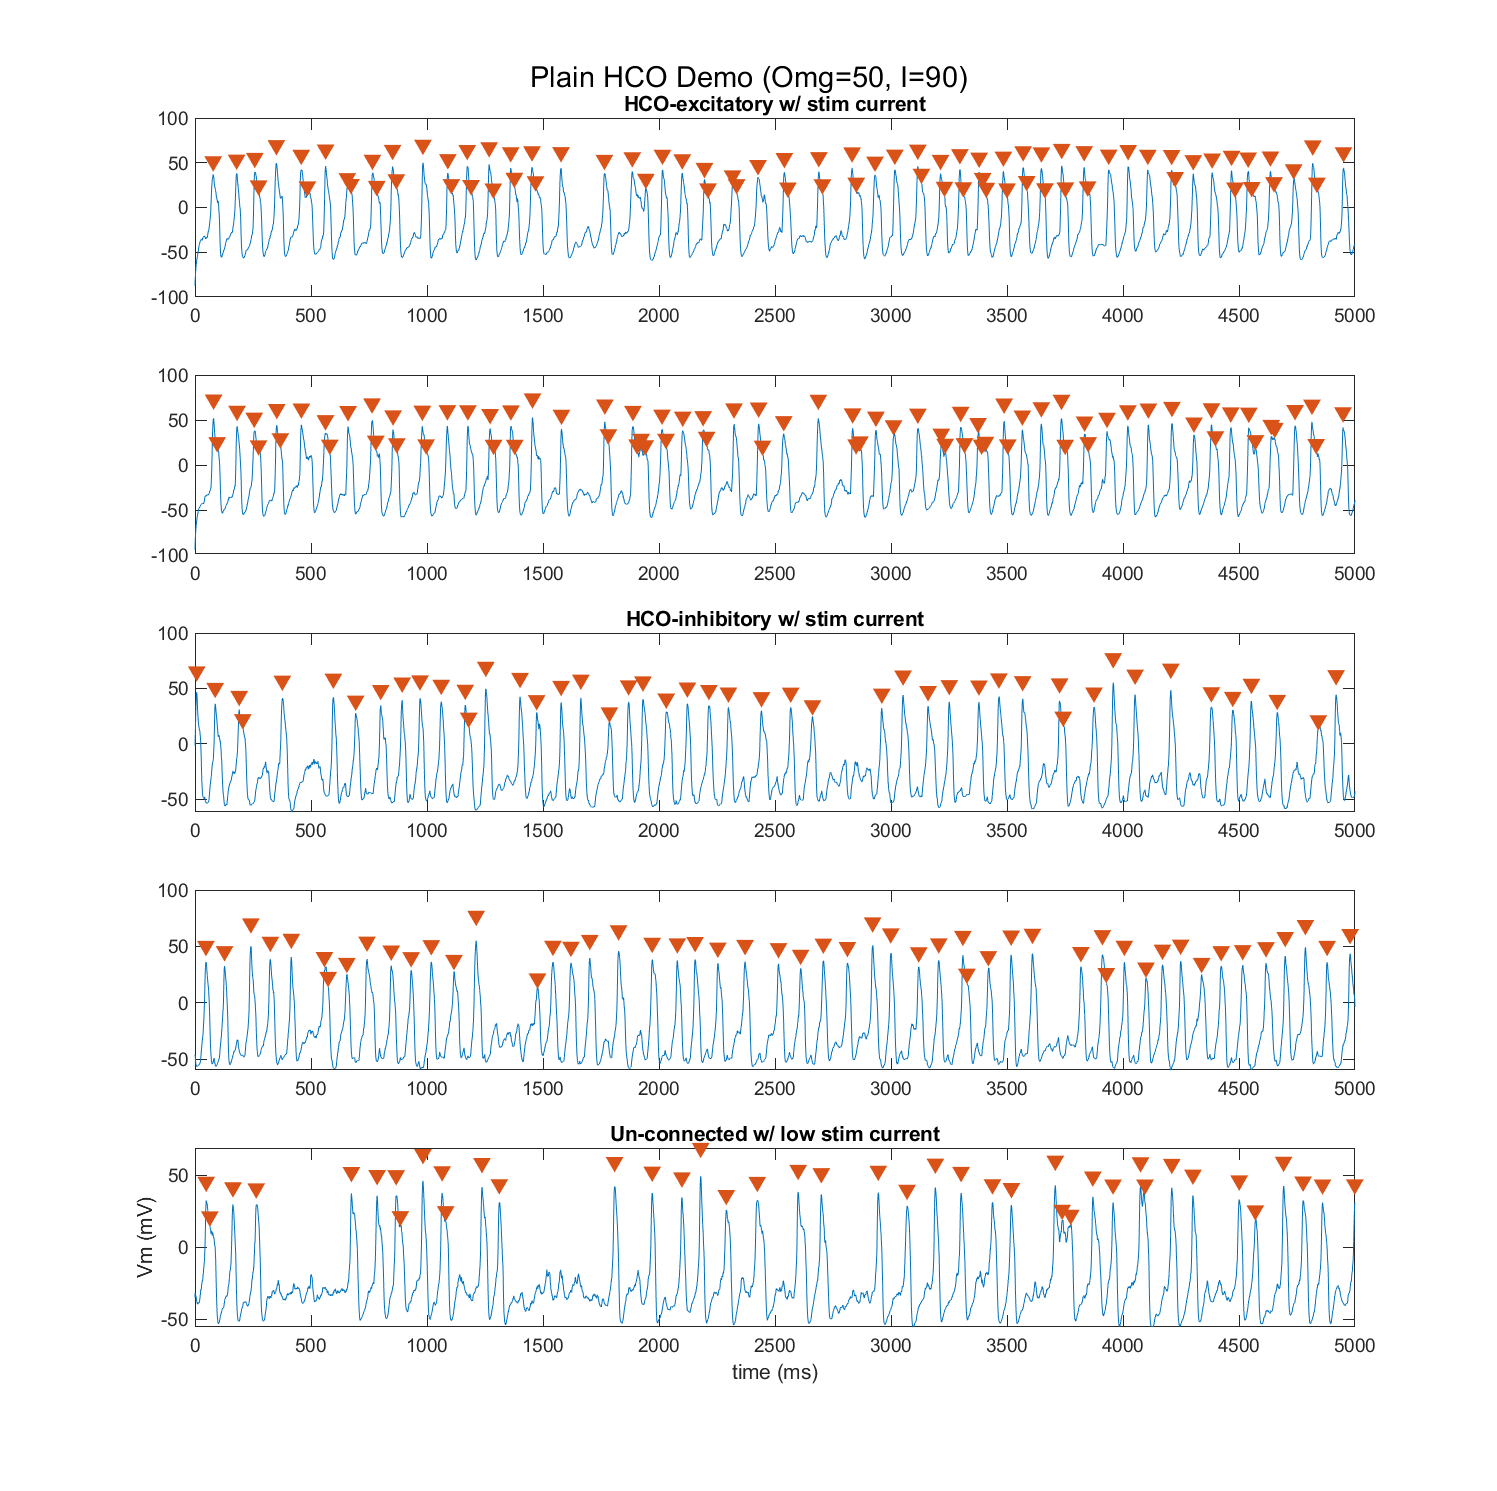
\includegraphics[width=.49\textwidth]{figs/old/Fx1_E_HCO_Om5e1_NB.png}
    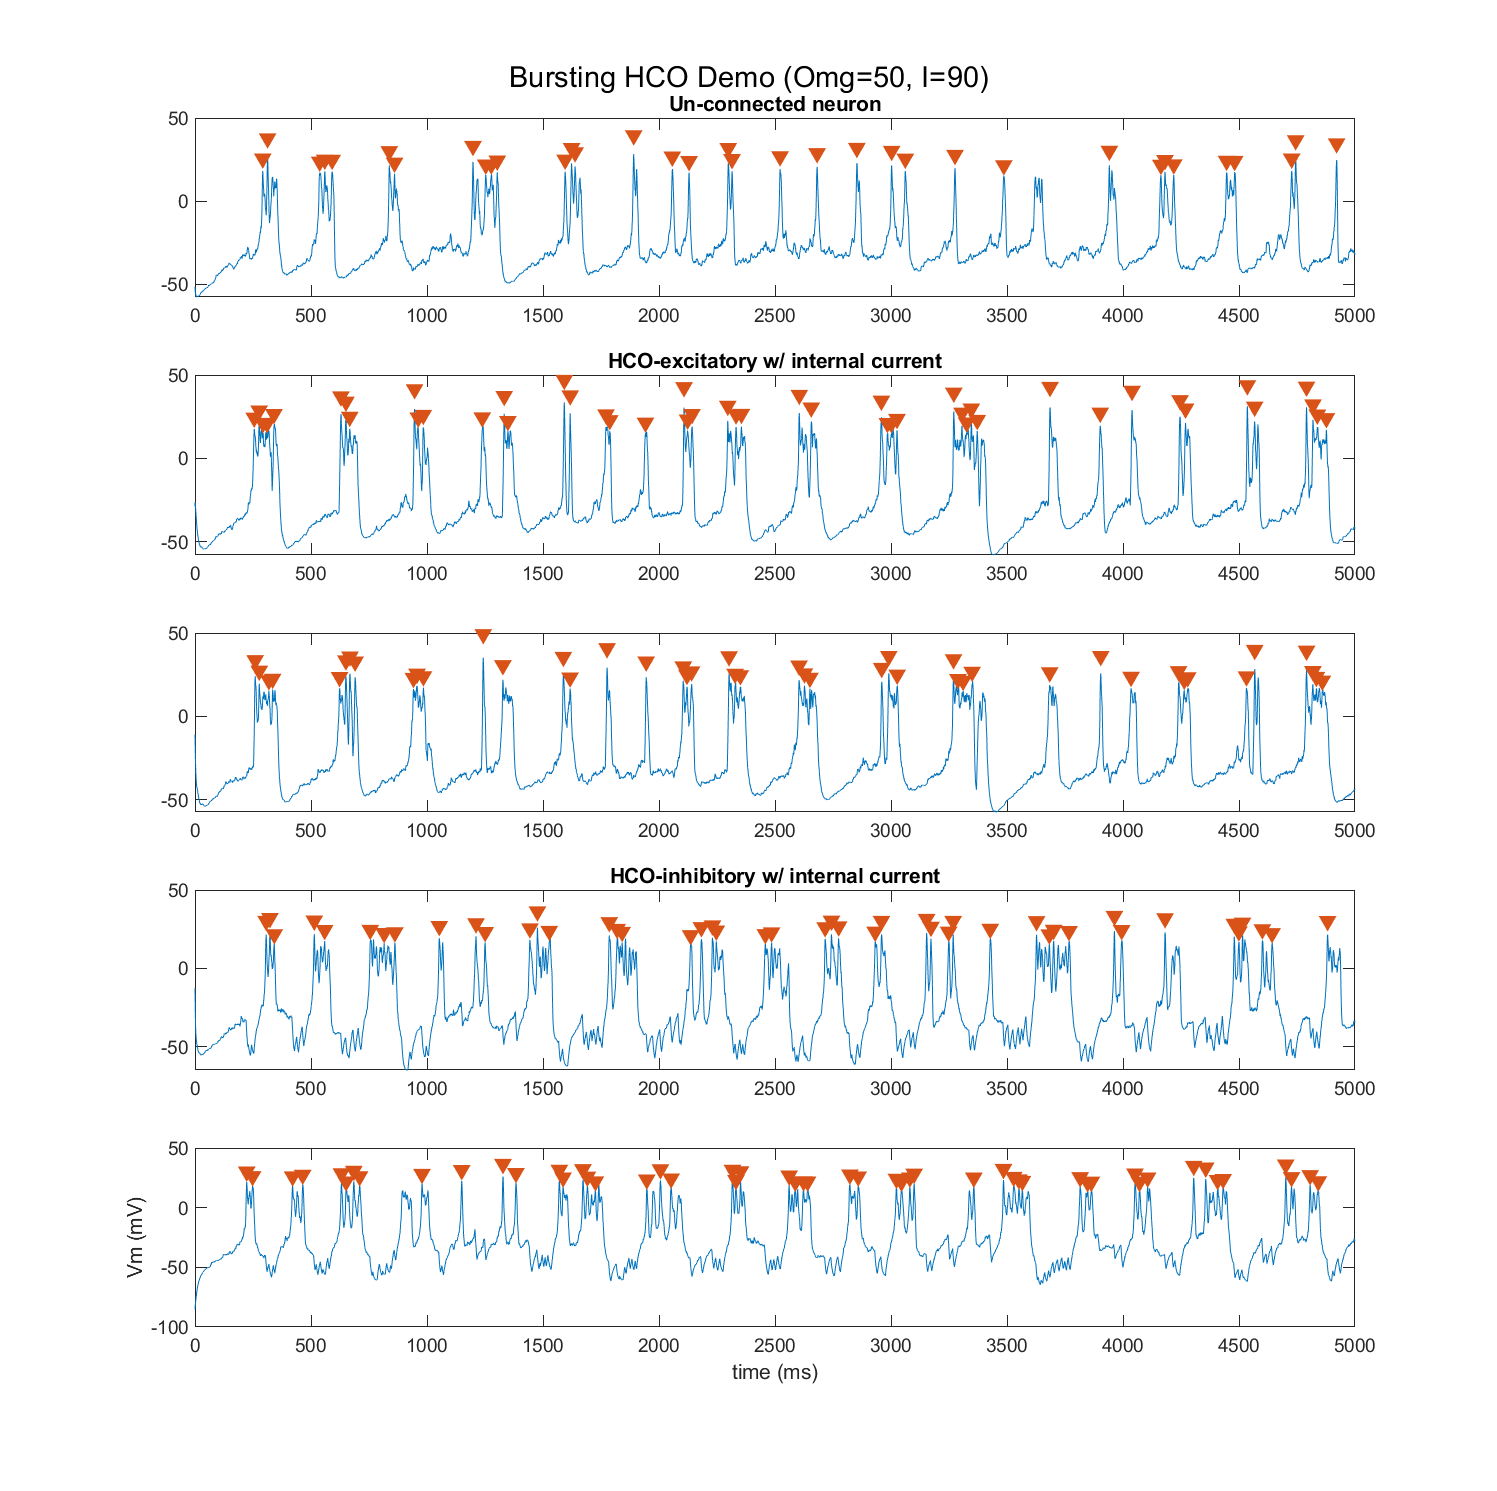
\includegraphics[width=.49\textwidth]{figs/old/Fx1_E_HCO_Om5e1_B.png}
    \vspace{-0.5cm} \caption{Stochastic HCO with Omega=50.}
  \end{subfigure}
\end{figure}

\begin{figure} \ContinuedFloat
  \centering
  \begin{subfigure}[b]{\textwidth}  
    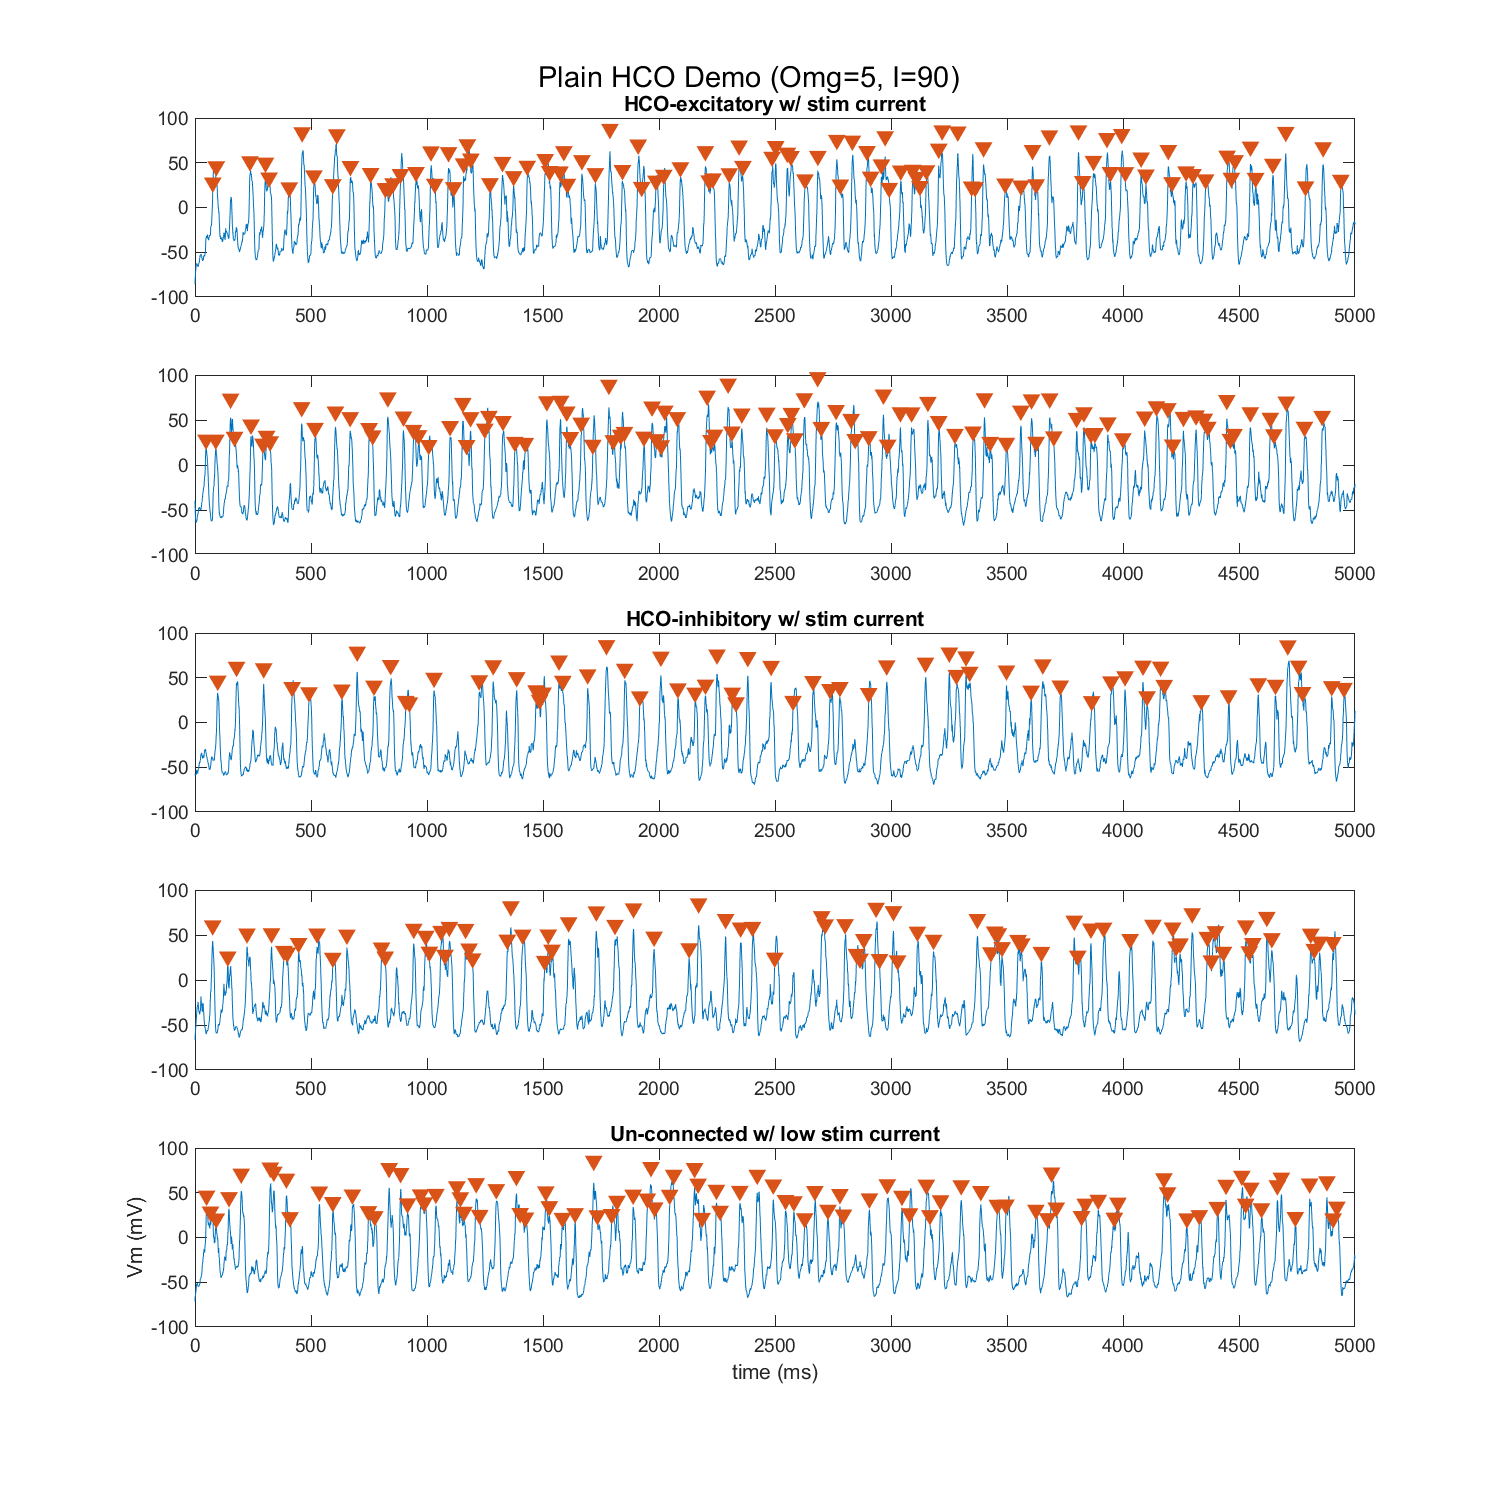
\includegraphics[width=.49\textwidth]{figs/old/Fx1_F_HCO_Om5e0_NB.png}
    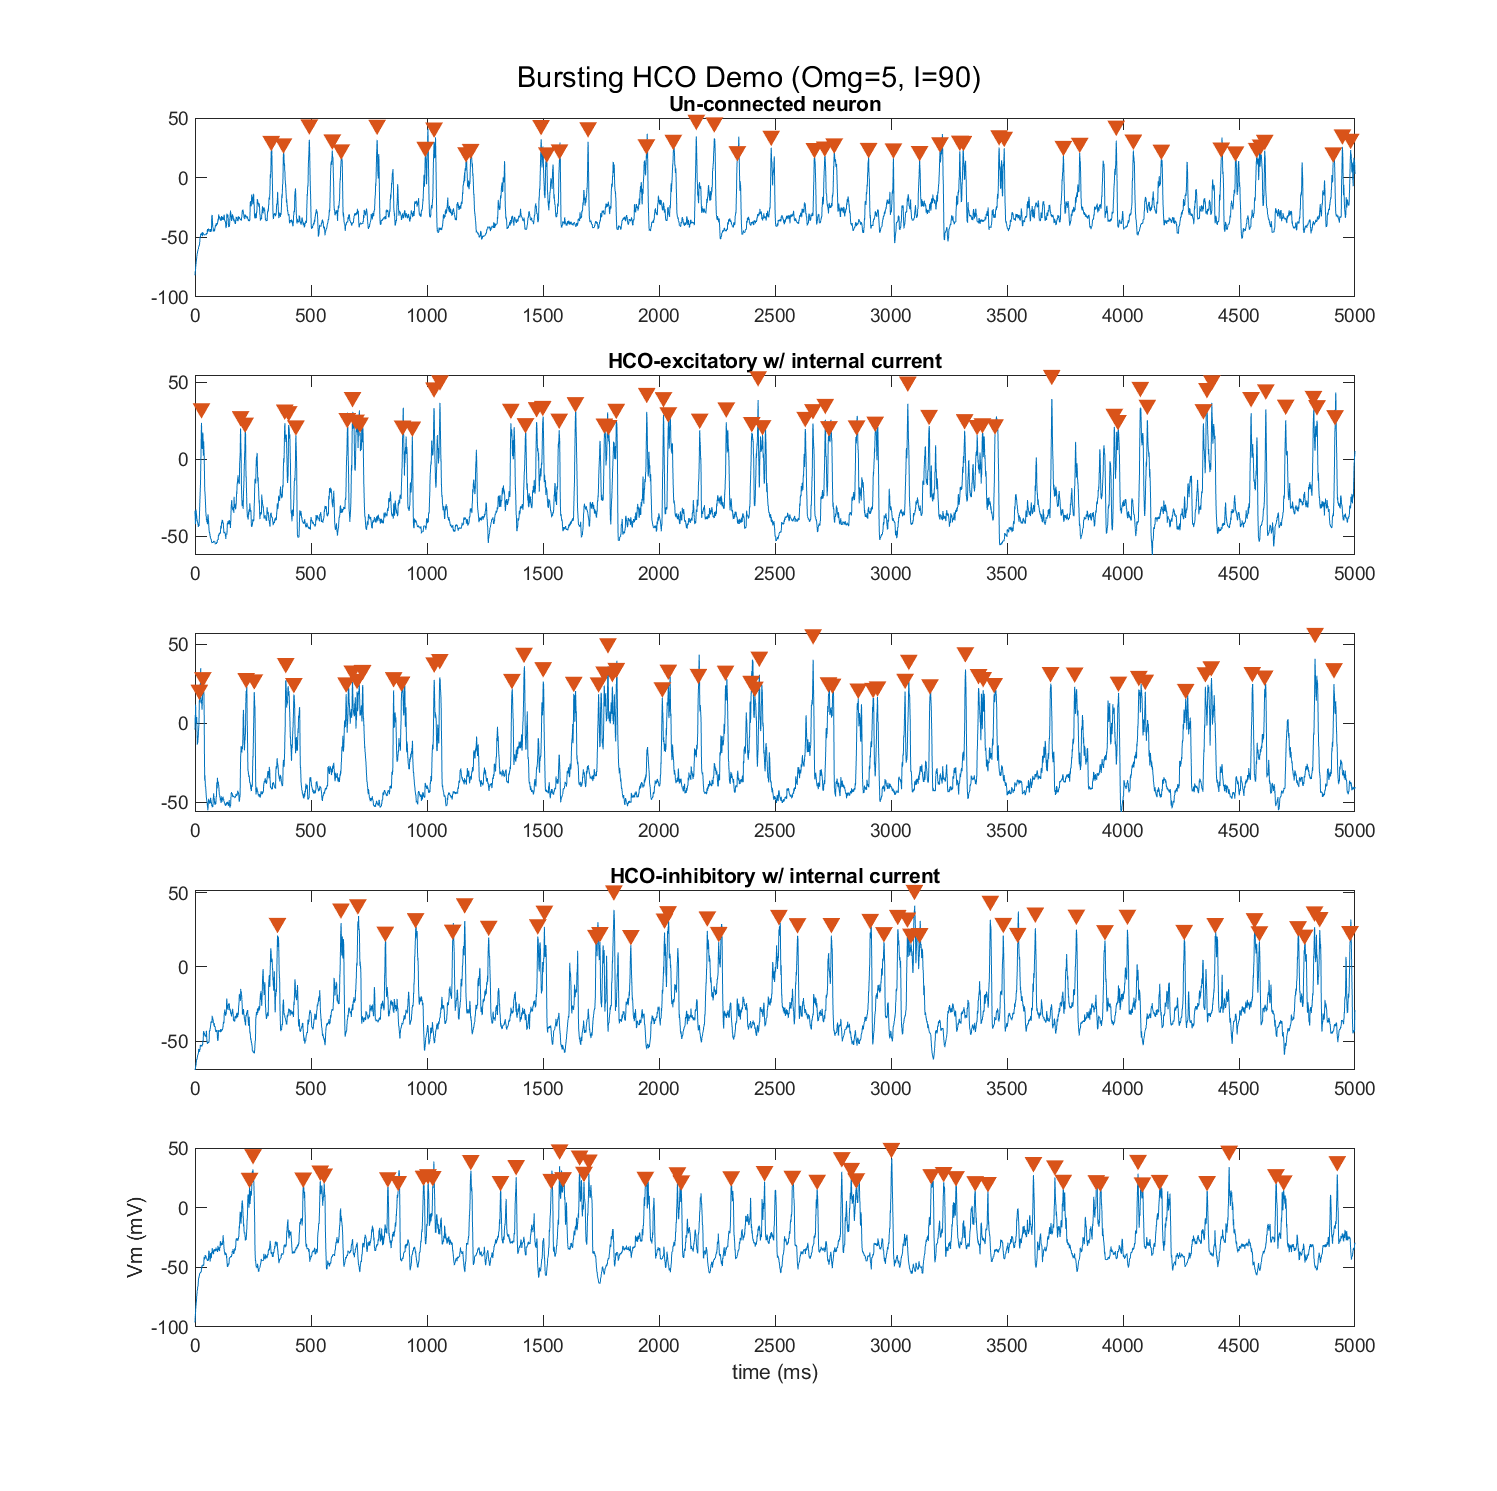
\includegraphics[width=.49\textwidth]{figs/old/Fx1_F_HCO_Om5e0_B.png}
    \vspace{-0.5cm} \caption{Stochastic HCO with Omega=5.}
  \end{subfigure}
  \vspace{-0.5cm} \caption{Single-Run Raw Plots }  \label{fig:figx1}
\end{figure}

\clearpage

\hypertarget{appendix-b-codes}{%
\section{Appendix B : Codes}\label{appendix-b-codes}}

\hypertarget{matlab-code-for-simulation}{%
\subsection{Matlab code for simulation}\label{matlab-code-for-simulation}}

\definecolor{mygreen}{RGB}{28,172,0}
\definecolor{mylilas}{RGB}{170,55,241}
\lstset{language=Matlab,%
    %basicstyle=\color{red},
    breaklines=true,%
    morekeywords={matlab2tikz},
    keywordstyle=\color{blue},%
    morekeywords=[2]{1}, keywordstyle=[2]{\color{black}},
    identifierstyle=\color{black},%
    stringstyle=\color{mylilas},
    commentstyle=\color{mygreen},%
    showstringspaces=false,%without this there will be a symbol in the places where there is a space
    numbers=left,%
    numberstyle={\tiny \color{black}},% size of the numbers
    numbersep=9pt, % this defines how far the numbers are from the text
    emph=[1]{for,end,break},emphstyle=[1]\color{red}, %some words to emphasise
    %emph=[2]{word1,word2}, emphstyle=[2]{style},    
}

\hypertarget{MLm}{%
\subsubsection{ML\_neurons : Parallel simulation of an array of neurons connected in a network}\label{MLm}}

\lstinputlisting{matlab_scripts/ML_neurons.m}

\hypertarget{MLnet}{%
\subsubsection{ML\_network : Initializing and simulating a network of ML neurons}\label{MLnet}}

(Note : ``Demo=1'' option in this function gives a demo of all HCO types.)

\lstinputlisting{matlab_scripts/ML_network.m}

\hypertarget{binlesscorrelation-plotting-gaussian-smoothed-spike-trains-and-computing-cross-correlation-between-two-traces.}{%
\subsubsection{BinlessCorrelation : Plotting gaussian smoothed spike-trains and computing cross-correlation between two traces.}\label{binlesscorrelation-plotting-gaussian-smoothed-spike-trains-and-computing-cross-correlation-between-two-traces.}}

\lstinputlisting{matlab_scripts/GetBinlessCorr.m}

\hypertarget{other-things-latex-figures-codes}{%
\subsection{Other things : LaTeX, Figures, Codes}\label{other-things-latex-figures-codes}}

\begin{itemize}
\tightlist
\item
  All Matlab simulation script, Matlab scripts for all figures, tex/md files for generating this report and figures files are available here :

  \begin{itemize}
  \tightlist
  \item
    \textless{}\href{https://github.com/shivanshdave/ML_HCO_sync}{GitHub-shivanshdave}\textgreater{}
  \end{itemize}
\end{itemize}

\hypertarget{references}{%
\section*{References}\label{references}}
\addcontentsline{toc}{section}{References}

\hypertarget{refs}{}
\begin{CSLReferences}{1}{0}
\leavevmode\hypertarget{ref-anderson15stochastic}{}%
Anderson, David F., Bard Ermentrout, and Peter J. Thomas. 2015. {``Stochastic Representations of Ion Channel Kinetics and Exact Stochastic Simulation of Neuronal Dynamics.''} \emph{Journal of Computational Neuroscience} 38 (1): 67--82. \url{https://doi.org/10.1007/s10827-014-0528-2}.

\leavevmode\hypertarget{ref-cdc18epilepsy}{}%
CDC. 2018. {``Epilepsy.''} https://www.cdc.gov/epilepsy/about/fast-facts.htm.

\leavevmode\hypertarget{ref-ermentrout10mathematical}{}%
Ermentrout, G. Bard, and David H. Terman. 2010. \emph{Mathematical {Foundations} of {Neuroscience}}. Vol. 35. Interdisciplinary {Applied Mathematics}. {New York, NY}: {Springer New York}. \url{https://doi.org/10.1007/978-0-387-87708-2}.

\leavevmode\hypertarget{ref-gonzalez-miranda14pacemaker}{}%
González-Miranda, J. M. 2014. {``Pacemaker Dynamics in the Full {Morris}{{Lecar}} Model.''} \emph{Communications in Nonlinear Science and Numerical Simulation} 19 (9): 3229--41. \url{https://doi.org/10.1016/j.cnsns.2014.02.020}.

\leavevmode\hypertarget{ref-higham08modeling}{}%
Higham, Desmond J. 2008. {``Modeling and {Simulating Chemical Reactions}.''} \emph{SIAM Review} 50 (2): 347--68. \url{https://doi.org/10.1137/060666457}.

\leavevmode\hypertarget{ref-izhikevich06bursting}{}%
Izhikevich, Eugene M. 2006. {``Bursting.''} \emph{Scholarpedia} 1 (3): 1300. \url{https://doi.org/10.4249/scholarpedia.1300}.

\leavevmode\hypertarget{ref-jutras10synchronous}{}%
Jutras, Michael J, and Elizabeth A Buffalo. 2010. {``Synchronous Neural Activity and Memory Formation.''} \emph{Current Opinion in Neurobiology}, Cognitive neuroscience, 20 (2): 150--55. \url{https://doi.org/10.1016/j.conb.2010.02.006}.

\leavevmode\hypertarget{ref-kruskal07binless}{}%
Kruskal, Peter B., Jessica J. Stanis, Bruce L. McNaughton, and Peter J. Thomas. 2007. {``A Binless Correlation Measure Reduces the Variability of Memory Reactivation Estimates.''} \emph{Statistics in Medicine} 26 (21): 3997--4008. \url{https://doi.org/10.1002/sim.2946}.

\leavevmode\hypertarget{ref-lecar07morrislecar}{}%
Lecar, Harold. 2007. {``Morris-{Lecar} Model.''} \emph{Scholarpedia} 2 (10): 1333. \url{https://doi.org/10.4249/scholarpedia.1333}.

\leavevmode\hypertarget{ref-mainen96influence}{}%
Mainen, Zachary F., and Terrence J. Sejnowski. 1996. {``Influence of Dendritic Structure on Firing Pattern in Model Neocortical Neurons.''} \emph{Nature} 382 (6589): 363--66. \url{https://doi.org/10.1038/382363a0}.

\leavevmode\hypertarget{ref-mormann03epileptic}{}%
Mormann, Florian, Thomas Kreuz, Ralph G Andrzejak, Peter David, Klaus Lehnertz, and Christian E Elger. 2003. {``Epileptic Seizures Are Preceded by a Decrease in Synchronization.''} \emph{Epilepsy Research} 53 (3): 173--85. \url{https://doi.org/10.1016/S0920-1211(03)00002-0}.

\leavevmode\hypertarget{ref-morris81voltage}{}%
Morris, C., and H. Lecar. 1981. {``Voltage Oscillations in the Barnacle Giant Muscle Fiber.''} \emph{Biophysical Journal} 35 (1): 193--213. \url{https://doi.org/10.1016/S0006-3495(81)84782-0}.

\leavevmode\hypertarget{ref-pikovsky07synchronization}{}%
Pikovsky, Arkady, and Michael Rosenblum. 2007. {``Synchronization.''} \emph{Scholarpedia} 2 (12): 1459. \url{https://doi.org/10.4249/scholarpedia.1459}.

\leavevmode\hypertarget{ref-rinzel98chapter7}{}%
Rinzel, John, and G. Bard Ermentrout. 1998. \emph{Chapter-7 : {Methods} in Neuronal Modeling: From Ions to Networks}. Edited by Christof Koch and Idan Segev. 2nd ed. Computational Neuroscience. {Cambridge, Mass}: {MIT Press}.

\leavevmode\hypertarget{ref-vanvreeswijk94when}{}%
Van Vreeswijk, Carl, L. F. Abbott, and G. Bard Ermentrout. 1994. {``When Inhibition Not Excitation Synchronizes Neural Firing.''} \emph{Journal of Computational Neuroscience} 1 (4): 313--21. \url{https://doi.org/10.1007/BF00961879}.

\leavevmode\hypertarget{ref-victor97metricspace}{}%
Victor, Jonathan D., and Keith P. Purpura. 1997. {``Metric-Space Analysis of Spike Trains: Theory, Algorithms and Application.''} \emph{Network: Computation in Neural Systems} 8 (2): 127--64. \url{https://doi.org/10.1088/0954-898X_8_2_003}.

\leavevmode\hypertarget{ref-who20epilepsy}{}%
WHO. 2020. {``Epilepsy.''} https://www.who.int/westernpacific/health-topics/epilepsy.

\leavevmode\hypertarget{ref-wilkinson19stochastic}{}%
Wilkinson, Darren James. 2019. \emph{Stochastic Modelling for Systems Biology}. Third edition. Chapman \& {Hall}/{CRC} Mathematical and Computational Biology. {Boca Raton}: {CRC Press, Taylor and Francis Group}.

\leavevmode\hypertarget{ref-yu00dynamical}{}%
Yu, Zhuojun, and Peter J. Thomas. n.d. {``Dynamical {Consequences} of {Sensory Feedback} in a {Half}-{Center Oscillator Coupled} to a {Simple Motor System}.''} {Unpublished}.

\end{CSLReferences}

\end{document}
